
\section*{\centering Reproducibility Summary}
% \textit{Template and style guide to \href{https://paperswithcode.com/rc2020}{ML Reproducibility Challenge 2020}. The following section of Reproducibility Summary is \textbf{mandatory}. This summary \textbf{must fit} in the first page, no exception will be allowed. When submitting your report in OpenReview, copy the entire summary and paste it in the abstract input field, where the sections must be separated with a blank line.
% }

\subsection*{Scope of Reproducibility}

In this work we perform a replication study of the paper \textit{Parameterized Explainer for Graph Neural Network}. The replication experiment focuses on three main claims: (1) Is it possible to reimplement the proposed method in a different framework? (2) Do the main claims with respect to the GNNExplainer hold? (3) Is the used evaluation method a valid method for explaining the classification decision by Graph Neural Networks? 

\subsection*{Methodology}

The authors' TensorFlow code was largely used as starting point for our reimplementation in PyTorch. However, large parts of the evaluation setup were missing and differences were found between the listed configurations in the paper and the code. As a result, our codebase contains a large portion of novel code and introduces a different method for tracking experimental configurations. Using the new codebase all experiments are replicated. In addition to this, a short ablation study is performed.

% Briefly describe what you did and which resources you used. For example, did you use author's code? Did you re-implement parts of the pipeline? You can also use this space to list the hardware used, and the total budget (e.g. GPU hours) for the experiments. 

\subsection*{Results}
Due to numerous inconsistencies between code and paper, it is not possible to replicate the original results using the paper alone. With help of the original codebase, a number of the original results can be retrieved. The main comparison claim of the paper, to improve over the preceding GNNExplainer, does hold. However, after performing the replication experiments, some questions regarding the validity of the used evaluation setup in the original paper remain. 


% Start with your overall conclusion --- where did your results reproduce the original paper, and where did your results differ? Be specific and use precise language, e.g. "we reproduced the accuracy to within 1\% of reported value, which supports the paper's conclusion that it outperforms the baselines". Getting exactly the same number is in most cases infeasible, so you'll need to use your judgement to decide if your results support the original claim of the paper.

\subsection*{What was easy}

The method proposed by the authors for explaining the Graph Neural Networks is easy to comprehend and intuitive. Re-implementation of the method is straightforward using a modern deep learning framework. The datasets used for the experimental setup were all provided together with their codebase. 

% Describe which parts of your reproduction study were easy. For example, was it easy to run the author's code, or easy to re-implement their method based on the description in the paper? The goal of this section is to summarize to a reader which parts of the original paper they could easily apply to their problem.

\subsection*{What was difficult}

The main difficulty arose from the difference between the experimental configurations discussed in the paper and implemented in the code. There were a number of small inconsistencies (eg. incorrect hyperparameter settings), but also some major ones (eg. using batch-normalization in training mode during evaluation). This issue was worsened by the fractured reporting of configurations in the code. 

% Describe which parts of your reproduction study were difficult or took much more time than you expected. Perhaps the data was not available and you couldn't verify some experiments, or the author's code was broken and had to be debugged first. Or, perhaps some experiments just take too much time/resources to run and you couldn't verify them. The purpose of this section is to indicate to the reader which parts of the original paper are either difficult to re-use, or require a significant amount of work and resources to verify.

\subsection*{Communication with original authors}
Contact was made with the authors on two occasions. During the first exchange the authors confirmed a number of clarifying questions and confirmed that the configurations as presented in the codebase were to be used instead of those provided in the paper. In the second exchange our reservations concerning the used experimental evaluation were conveyed to the authors. The authors did not share our concerns. 
% Briefly describe how much contact you had with the original authors (if any).

\newpage % Simulate a very long abstract
\section{Introduction}
Graph Neural Networks (GNNs) emerged as state-of-the-art models in machine learning, capturing both graph structure and node features through recursively incorporating a graph's previous node information. GNNs are able to deliver state-of-the-art performances in matters such as graph/node classification and link prediction.

As for most Neural Networks, the 'reasoning' towards classification inside GNNs is not intuitive to humans. The authors of the paper \textit{GNNExplainer: Generating Explanations for Graph Neural Networks} \cite{ying2019gnnexplainer} address this problem and try to solve it by introducing \textsc{GNNExplainer}; an optimization task that maximizes the mutual information between a GNN's prediction and a distribution of possible sub-graph structures. The GNNExplainer's algorithm can identify the sub-graph and node structure responsible for a given classification.
Based on the work done in \cite{ying2019gnnexplainer}, Luo, D. et al. claim to have further developed GNNExplainer in their paper \textit{Parameterized Explainer for Graph Neural Network} \cite{luo2020parameterized}. The paper introduces \textsc{PGExplainer}; a general parameterized explainer that applies to any GNN based models in both transductive and inductive settings. 

The authors of the paper first formulate the learning objective of PGExplainer. Using the same datasets as \cite{ying2019gnnexplainer}, they claim to outperform GNNExplainer up to $24.7\%$ in Area under the ROC Curve (AUC) \cite{Hanley1982roc-auc} score. Furthermore the authors state that PGExplainer can speed up computations up to $108$ times faster than GNNExplainer. These and further claims made in the PGExplainer paper will be evaluated in this report by replicating and extending the performed evaluation in a replication study.

\paragraph{Scope of reproducibility}\label{sec:scope}
The focus of our reproducibility study is on the experimental comparison between the PGExplainer and the preceding GNNExplainer. The authors of the original PGExplainer paper include a number of other benchmarks in their evaluation, but focus their comparison primarily on the GNNExplainer. For this reason it makes sense for us to do the same. 

In contrast to the original paper, we will base our entire comparison on reimplementations of both methods. In the original paper, the authors partly copy the results from the GNNExplainer and partly use their own re-implementation to obtain the GNNExplainer scores. In communication the authors stated that the decision to partly copy the results was made due to lackluster results in their own re-implementation. As the quality of an explanation is highly dependent on the model it aims to explain, we believe that it would be beneficial to re-implement both methods in the same framework and perform their evaluation on equal footing. We will use PyTorch as the framework for doing so. 

For the reimplementation of the PGExplainer the authors' own TensorFlow-based codebase provided in their paper will be used as the main starting-point. However, during inspection of the codebase, we found that there are a number of significant differences between the configurations used for both the trained models that we wish to explain and the PGExplainer itself between what is described in the paper and what is actually implemented in the code. After discussing with the authors, the conclusion was reached that the configurations used in the code should serve as the starting point for the replication. Part of our reproduction experiment will focus on validating if these are indeed the correct configurations. 
In short, our replication experiment aims to validate the following aspects of the original paper.

\begin{enumerate}[]
    \item Given the original codebase and configuration files provided therein, is it possible to reimplement the PGExplainer method using a different framework? And if so, are the provided configurations sufficient to obtain the presented quantitative, qualitative and efficiency results. 
    \item The authors claim that their PGExplaimer greatly improves over the previously proposed GNNExplainer. We aim to validate that this claim holds with both methods evaluated using the same framework and evaluation. 
    \item Evaluation of explanation methods is notoriously hard. We wish to validate if the evaluation method used in the original paper is a sound approach for doing so.
\end{enumerate}

% we reimplement the PGExplainer using PyTorch. By doing so, a more direct comparison can be made using the models trained for the GNNExplainer. More specifically, we aim to reproduce and verify PGExplainer results, reevaluating the PGExplainer qualitatively, quantitatively, and its efficiency using a framework that it was not initially designed for.

% In this work we check the reproducibility of the PGExplainer paper on two levels. First, we perform a \textit{simple} replication experiments of the evaluation performed in the paper itself. During inspection of the code base, we found that there are a number of significant difference between the configurations used for both the trained models that we wish to explain and the PGExplainer itself between what is described in the paper and what is actually implemented in the code. After discussing with the authors, the conclusion was reached that the configurations used in the code should serve as the starting point for the reproducibility check. During the replication experiment, we wish to validate that the configurations provided by the code base can be trusted. 

% The second objective is to perform an extended reproduction check. While re-implementing the evaluation of the PGExplainer, a number of undefined strong assumptions were observed that could significantly impact the models evaluation. For example, the evaluation is only performed over a subset of the available samples. Most of which are part of the training set. During the extended reproduction check, we validate that the improvements seen in the paper are not a result of these assumptions. 

% Additionally, the extended reproducibility check is used to validate the influence of the used frameworks for the evaluation. The authors implemented the PGExplainer method using the TensorFlow \cite{tensorflow2015-whitepaper} library, while the GNNExplainer method is implemented using PyTorch. Due to a lack of the authors' motivation to proceed using TensorFlow instead of PyTorch, we are uncertain about evaluated explanations generated for the same model. This uncertainty is strengthened by the authors choice not to include code of the baseline models, and reuse scores from the GNNExplainer paper in the quantitative evaluation. As the quality of an explanation is highly dependent on the model it aims to explain, we re-implement the PGExplainer using PyTorch. By doing so, a more direct comparison can be made using the models trained for the GNNExplainer. More specifically, we aim to reproduce and verify PGExplainer results, reevaluating the PGExplainer qualitatively, quantitatively, and its efficiency using a framework that it was not initially designed for. 

The remainder of this work will be structured as follows. In the next section we will provide the needed background on the PGExplainer. Following this, we will provide a short overview of the codebase accompanying this reproduction. In section \ref{sec:replication}, we will discuss the original experimental setup in depth and highlight some key components not discussed in the original paper. Section \ref{sec:results} will present the replicated results and compare them to the original paper. Based on the highlighted components in section \ref{sec:replication} and some results presented in section \ref{sec:results}, section \ref{sec6} will raise some question regarding the evaluation setup used. In the last section, we will summarize our replication. 

% The remainder of this work will be structured as follows. In the next section, we will provide the needed background on the PGExplainer. Following this, we will provide a short overview of the code base accompanying this reproducibility check. In section 4 and 5 we will present the replication and extend reproduction check respectively. Each section will include an overview of the experimental setup, the obtained results as well as an discussion of these results. In the last section, the conclusion, we will summarize the reproducibility check and provide an overview of the main issues found. 

\section{PGExplainer}\label{sec:PGE}
The authors start by dividing an input graph $G_o$ in two subgraphs, such that $G_o = G_s + \Delta G$. $G_s$ represents the \textit{explanatory graph} that makes important contributions towards the graph classification, while $\Delta G$ represents the remainder of the initial graph. The main task therefore is to find the optimal subgraph $G_s$. This is achieved through Mutual Information ($MI$) maximization:
\begin{align}
    \max _{G_{s}} \operatorname{MI}\left(Y_{o}, G_{s}\right)=H\left(Y_{o}\right)-H\left(Y_{o} \mid G=G_{s}\right),
\end{align}
Which uses the GNN's classification prediction $Y_o$ and its input $G_o$. The MI maximization is done by deducting the conditional entropy from the marginal entropy. Which is equivalent to minimizing the conditional entropy.

To avoid having an exploding exponential amount of candidates, the authors assume the explanatory graphs used are Gilbert random graphs \cite{Gilbert1959}, where selections of edges from the original input graph $G_o$ are conditionally independent to each other. 
Using relaxation, the learning objective is rewritten as
\begin{align}
    \min _{G_{s}} \mathbb{E}_{G_{s}}\left[H\left(Y_{o} \mid G=G_{s}\right)\right] \approx \min _{\Theta} \mathbb{E}_{G_{s} \sim q(\Theta)}\left[H\left(Y_{o} \mid G=G_{s}\right)\right],
\end{align}
where $q(\Theta)$ is the distribution of the parameterized explanatory graph. Each graph edge obtains a continuous variable in range $(0, 1)$.

A random graph $\hat{G}_s$ is sampled from edge distributions and fed to the trained GNN model obtaining prediction $\hat{Y}_s$. Following \cite{ying2019gnnexplainer}, the authors modify the conditional entropy with cross-entropy $H(Y_o,\hat{Y}_s)$, where $\hat{Y}_s$ is the prediction of the GNN model with $\hat{G}_s$ as input. Using Monte Carlo approximation, the learning objective becomes
\begin{align}
    \min _{\Omega}-\frac{1}{K} \sum_{k=1}^{K} \sum_{c=1}^{C} P_{\Phi}\left(Y=c \mid G=G_{o}\right) \log P_{\Phi}\left(Y=c \mid G=\hat{G}_{s}^{(k)}\right),
\end{align}
with $\Phi$ as the parameters in the trained GNN, $K$ as the number of sampled graphs, $C$ as the number of labels and $\hat{G}_s^{(k)}$ the $k$-th sampled graph, parameterized by $\Omega$.

Furthermore, PGExplainer is used to collectively provide explainations for multiple instances $\mathcal{I}$. The authors present the learning objective of this set of instances as follows.
\begin{align}
    \min _{\Psi}-\sum_{i \in \mathcal{I}} \sum_{k=1}^{K} \sum_{c=1}^{C} P_{\Phi}\left(Y=c \mid G=G_{o}^{(i)}\right) \log P_{\Phi}\left(Y=c \mid G=\hat{G}_{s}^{(i, k)}\right)
\end{align}
Here $\Psi$ are parameters in the explanation network, $G^{(i)}$ the input graph and $\hat{G}^{(i, k)}$ the $k$-th sampled graph for the $i$-th instance.
Using the above, the authors consider two explainer instances; one for node classification and one for graph classification. Both cases use a MLP parameterized by $\Psi$.
\section{Reimplementation of code}\label{sec:3}
This section shortly summarizes the main structure of the code accompanying this reproducibility check and provides the information needed to reproduce the experiments presented. Our reimplementation of the PGExplainer is based on the PyTorch \cite{PyTorch} framework. More specifically, it uses the third party extension of PyTorch for Graph Neural Networks called PyTorch-Geometric \cite{PyTorch-Geometric}. 

The codebase is structured for the two main tasks performed in this paper; training the GNNs that will be explained by the PGExplainer and performing a replication of the original experiments. Additional scripts are included for performing the evaluations presented in the appendix. Each script is self-contained, handling things such as loading the dataset, loading the correct model and setting the hyperparameters. Each of these things are predefined in \texttt{json} configuration files. 

\subsection{Experiment configuration files}
The codebase contains a large number of predefined configuration files. These configuration files are the main working horse for making the experiments presented in this work reproducible. There are two different types of configurations, one for each of the two main tasks mentioned previously. Shared between tasks is the common occurrence of the dataset, model and seed used. If a task is to be performed a number of times to achieve an average, the seed is replaced with a list of seeds. A full description of the configuration file setup can be found in Appendix \ref{appendix:A}. 

As these configuration files provide a reliable source for all relevant information needed to perform our evaluation, we will---for the remainder of this paper---only disclose the information needed to comprehend the experiment. For details irrelevant to understanding the results---e.g. the used learning rate and specific framework versions---we refer to the provided configuration and codebase\footnote{\url{https://github.com/LarsHoldijk/RE-ParameterizedExplainerForGraphNeuralNetworks}}. We understand that this breaks the papers self-containment. However, we believe that regarding the balance between page restrictions and replicability completeness, separating the concern of replicability from paper to codebase is the correct way to go. A single source of replicability information also prevents inconsistencies between the paper and the code base. As the paper under consideration will highlight, this is a concern.
\section{Experiment Setup}\label{sec:replication} 
In this section we will introduce the setup of the experimental evaluation performed by the authors of the PGExplainer. While replicating their evaluation, we found that a number of steps were making assumptions that were not well documented. This includes the samples used for calculating the AUC score. In this section we will spend time on these steps. Additionally, some minor mistakes made in the original evaluation were rectified during our reproduction. These changes will also be highlighted here.

The experimental setup used by the authors of the PGExplainer follows that of the GNNExplainer \cite{ying2019gnnexplainer} with a number of extensions. To clarify, the authors' proposed method serves the purpose of explaining the classification decision of a GNN. Hence, the experiments used to evaluate the PGExplainer focus on the explanations provided by the PGExplainer for the underlying model. Specifically, the evaluation is repeated for six different datasets, and thus, for six different underlying models. The six datasets span two different classification tasks; node-classification and graph-classification. 

\subsection{Datasets \hfill \texttt{[datasets/dataset\_loaders.py]}}\label{sec:datasets}
The node classification task is performed using four synthetic datasets (a-d). All of which are first introduced in the GNNExplainer paper \cite{ying2019gnnexplainer}. The graph classification task is performed using two datasets (e-f), one synthetic and one real.

A reoccurring concept in all synthetic datasets is the so called \textit{motif}. Motifs are highly structured subgraphs---e.g. 9 nodes connected in a 2D grid. These subgraphs are then expanded by attaching them to a randomly generated graph of a different structural form---e.g. Barabasi-Albert (BA) graph \cite{Barabasi99emergenceScaling} or trees. Motifs play a crucial role in determining ground-truth explanations for our evaluations, as we will see later.
% All six datasets are specified and visualised in Table \ref{tab:results} (Appendix \ref{appendix:A}) \cite{luo2020parameterized}.

(a) The BA-Shapes dataset consists of single base BA-graph with 300 nodes, 80 “house”-structured motifs---each attached to random BA nodes---and some extra randomly added edges. (b) BA-Community closely resembles BA-Shapes, connecting two BA-Shapes and utilizing a Gaussian distributions for each BA-Shape to sample node features. (c) Tree-Cycles adopts an $8$-level balanced binary tree as the base graph with a set of $80$ six-node cycle motifs attached to randomly selected nodes. (d) The Tree-Grids dataset is similar to Tree-Cycles, replacing cycle motifs with $3\times 3$ grid motifs. (e) The authors constructed the BA-2motifs dataset consisting of $1000$ BA graphs. Half of the graphs contain "house" motifs, the other half contain five-node cycle motifs attached to the BA graph. These two types of graphs serve as the two classes for the dataset. (f) The real-life Mutagenicity dataset copied from \cite{ying2019gnnexplainer}, consisting of $4337$ molecule graphs. These should be classified as either mutagenic or nonmutagenic.
% All base nodes are labelled $0$, the nodes constructing the "house"'s top, middle and bottom are labelled $1$, $2$ and $3$ respectively. 
% In BA-Community nodes are labeled based on their structural roles and community memberships, leading to $8$ classes in total.


% \begin{enumerate}[(a)]
%     \item The BA-Shapes dataset consists of single base Barabasi-Albert (BA) graph \cite{Barabasi99emergenceScaling} with 300 nodes, 80 “house”-structured motifs---each attached to random BA nodes---and some extra randomly added edges. All base nodes are labelled $0$, the nodes constructing the "house"'s top, middle and bottom are labelled $1$, $2$ and $3$ respectively. 
%     \item BA-Community closely resembles BA-Shapes, connecting two BA-Shapes and utilizing a Gaussian distributions for each BA-Shape to sample node features. In BA-Community nodes are labeled based on their structural roles and community memberships, leading to $8$ classes in total.
%     \item Tree-Cycles adopts an $8$-level balanced binary tree as the base graph with a set of $80$ six-node cycle motifs attached to randomly selected nodes.
%     \item The Tree-Grids dataset is similar to Tree-Cycles, replacing cycle motifs with $3\times 3$ grid motifs.
%     \item The authors constructed the BA-2motifs dataset consisting of $1000$ BA graphs. Half of the graphs contain "house" motifs, the other half contain five-node cycle motifs attached to the BA graph. These two types of graphs serve as the two classes for the dataset.
%     \item The real-life Mutagenicity dataset copied from         \cite{ying2019gnnexplainer}, consisting of $4337$ molecule graphs. These should be classified as either mutagenic or nonmutagenic.
% \end{enumerate}


% In order to compare and evaluate results, the authors use the four datasets found in \cite{ying2019gnnexplainer}; BA-Shapes (1), BA-Community (2), Tree-Cycles (3), and Tree-Grids (4). Additionally, they construct a fifth graph classification dataset, BA-2motifs (5). All five datasets are also specified and visualised in Table \ref{tab:dataset_info} and Table \ref{tab:results} \cite{luo2020parameterized}.
% (1) The BA-Shapes dataset consists of single base Barabasi-Albert (BA) graph \cite{Barabasi99emergenceScaling} with 300 nodes, 80 “house”-structured motifs---each attached to random BA nodes---and some extra randomly added edges. All base nodes are labelled $0$, the nodes constructing the "house"'s top, middle and bottom are labelled $1$, $2$ and $3$ respectively. 
% (2) BA-Community closely resembles BA-Shapes, connecting two BA-Shapes and utilizing a Gaussian distributions for each BA-Shape to sample node features. In BA-Community nodes are labeled based on their structural roles and community memberships, leading to $8$ classes in total.
% (3) Tree-Cycles adopts an $8$-level balanced binary tree as the base graph with a set of $80$ six-node cycle motifs attached to randomly selected nodes.
% (4) The Tree-Grids dataset is similar to Tree-Cycles, replacing cycle motifs with $3\times 3$ grid motifs.
% (5) The authors constructed the BA-2motifs dataset consisting of $1000$ BA graphs. Half of the graphs contain "house" motifs, the other half contain five-node cycle motifs attached to the BA graph. These two types of graphs serve as the two classes for the dataset.
% (6) Finally, they include the real-life MUTAG dataset copied from \cite{ying2019gnnexplainer}, consisting of $4337$ molecule graphs. These should be classified as either mutagenic or nonmutagenic.


% \begin{table}[h]
%     \centering
%     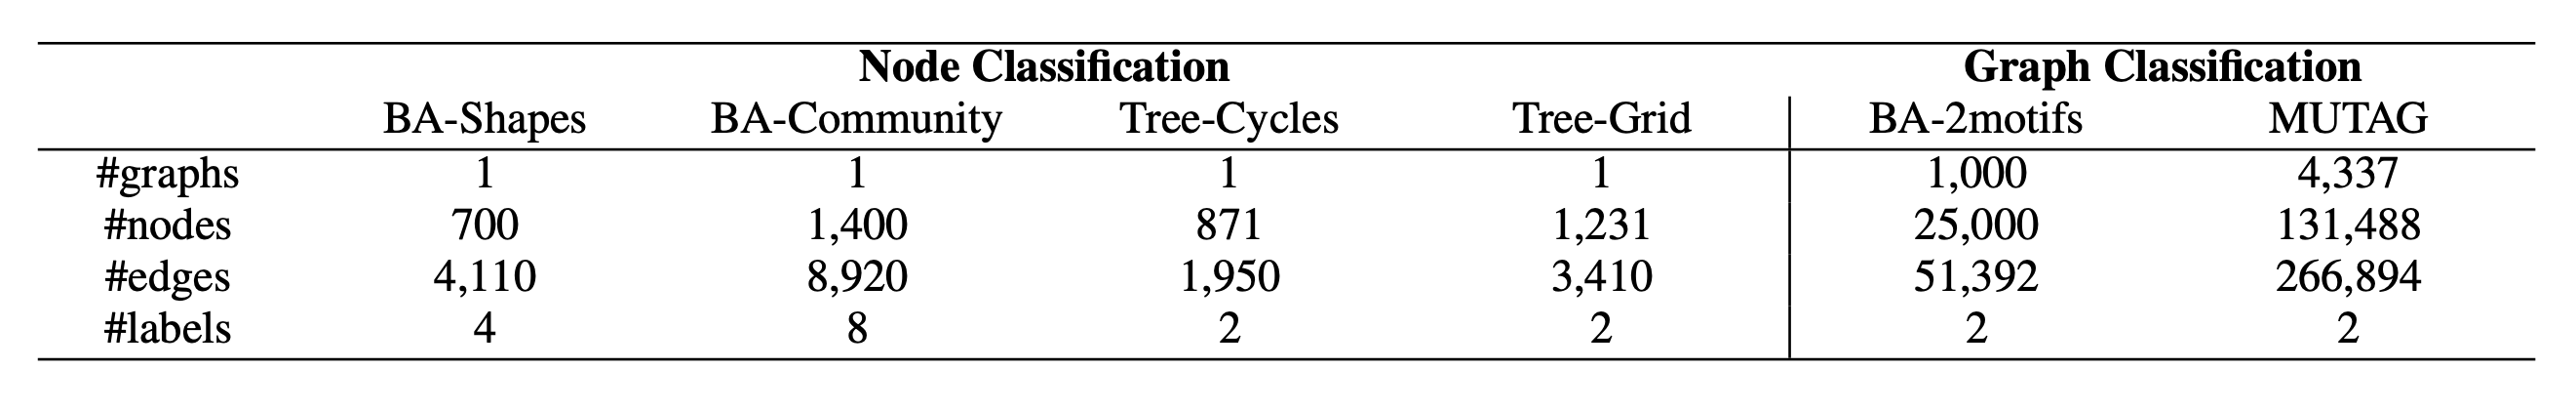
\includegraphics[width=1\linewidth]{imgs/dataset_info.png}
%     \caption{Original paper's dataset statistics \cite{luo2020parameterized}}
%     \label{tab:dataset_info}
% \end{table}

\subsection{Model \hfill \texttt{[models/GNN\_paper.py]}}
There are a number of large differences between the implementation of the models trained for each dataset and how they are described in the paper. These changes are different between the node and graph classification tasks. 

\paragraph{Node classification}
The authors describe the model for node classification to be three consecutive Graph Convolution layers feeding directly into the fully connected classification. The model in the codebase however first concatenates the three intermediate outputs of the Graph Convolution layers before using this enlarged embedding as the input for the fully connected classification layer. The coded version of the models is similar to what is used for evaluation in the GNNExplainer paper \cite{ying2019gnnexplainer}. To keep the evaluation consistent, we will therefore use the coded model version instead of the one described in the paper for our evaluation. Moreover, we were not able to get the model described in the paper to train to the same accuracy using the provided hyperparameters. 

In addition to the architecture change, we found the node classification models to use an undocumented batch normalization layer after the first and second Graph Convolution layer. Unfortunately, the original codebase contained an error that resulted in these batch-normalization layers being kept in training mode during evaluation. This observation was confirmed by the authors in communication and has since been resolved. In the same communication the authors expressed that to be able to reproduce their results, the batch normalization layers will have to be kept in training mode. We believe that this will compromise the usability of our reproducibility experiment and therefore decided to remove the batch normalization layers all together. For completeness full replication of the authors evaluation with a model containing batch normalization is included in Appendix \ref{appendix:batch_norm}.

\paragraph{Graph classification}
The graph classification models are more in line with the models described in the paper than the node classification models. The difference is the use of both max and mean pooling over the output of the final Graph Convolution layer. These two pooling types are concatenated to form inputs for fully connected layers.  

% In contrast to what is described in the paper, the model for which the PGExplainer provides explanations is considerably different from the model used in the GNNExplainer paper. Most notably, the authors included additional batch normalization layers for the first and second Graph Convolution layer. In addition to this, the implemented model does also not follow the general model structure as defined in the paper. Instead of using consecutive 3 Graph convolution layers feeding directly into the fully connected classification layer, the coded model first concatenates the three outputs of the GC layers before feeding it. 

% - Describe the model that they implemented in their code
%     - same as GNNExplainer, with additional batch normalization
% - In contrast to what is defined in the paper, the layers are concatenated
% - Use of both max and mean pooling in code, but not paper
% \paragraph{Training}
%     - As described in paper
%     - Main difference in code is longer training of the Graph classification models

\subsection{Evaluation metrics \hfill \texttt{[tasks/replication.py]}}

For each dataset, the explanations are evaluated using three broad categories; quantitative, qualitative and efficiency.

\subsubsection{Quantitative evaluation \hfill \texttt{[evaluation/AUCEvaluation.py]}}
For each dataset the explanations provided by the PGExplainer are compared to ground-truth explanations. These ground-truths describe for each sample which edges should or should not be included in the explanation. Using this methodology, the quantitative evaluation can be performed similar to a binary classification task. For this reason, the authors present the quantitative score using the AUC scoring metric. 

\paragraph{Ground Truth }
For node classification the ground-truth explanation is determined globally---i.e. for all node samples the edges have the same ground-truth explanation label. Specifically, for each edge it is determined if the two nodes it connects are part of a motif. When this is the case, the edge is labelled as positive for the ground-truth explanation. Otherwise, the edge is labelled as negative for the ground-truth explanation. For graph classifications this is dependent on the dataset used and how the ground-truth explanations are generated. For the BA-2motif dataset, being synthetic, this is done the same way as for the node datasets. The only difference being that the process is repeated for every graph in the dataset. As there are no motifs defined for the Mutagenicity dataset, the ground-truth labels can not be defined based on them. Instead, for this dataset edge labels are used, as provided by the original dataset repository\footnote{https://ls11-www.cs.tu-dortmund.de/staff/morris/graphkerneldatasets}. 

\paragraph{AUC score}
With the explanation mask provided by the PGExplainer and the ground-truths defined as above, the AUC score can be computed. However, there are a few important notes to consider when computing the AUC score. First, for the node classification datasets, the explanation mask is only determined for a 3-hop graph around each node. This is done because the GCN model only contains three layers. Second, only the nodes that are part of a motif are used in the AUC computation. This is because there is no real definition of ground-truth for the nodes outside the motifs. This evaluation design choice is further discussed in Sec.\,\ref{sec6}. Third, for the BA-2Motif dataset only a subset of the graphs is used to determine the AUC score, this is done to reduce computation time. Lastly, for the Mutagenicity dataset only the mutagenic graphs have a valid ground-truth interpretation. Hence, the AUC is determine using only these graphs. Of these four considerations, only the last is mentioned in the original paper. 

\paragraph{Comparison} The authors compare their method against four baselines; a gradient-based model (GRAD) \cite{ying2019gnnexplainer}, a graph attention network (ATT) \cite{velivckovic2017graph} and Gradient \cite{pope2019explainability}. With the exception of the scores presented for the graph-classification datasets, the scores presented are reused from the PGExplainer paper (see Table \ref{tab:results}). In communication with the authors, it was mentioned that the reimplementation of these explainers by the authors had resulted in lackluster results. For this reason the decision was made to use the original scores by the original authors. 

For our replication of the evaluation we focus our comparison on the GNNExplainer. This method is the most similar and was a major inspiration for the PGExplainer. In contrast the the original evaluation, we do perform the comparison using our own re-implementation of the GNNExplainer. Our re-implementation of this method is largely inspired by the implementation in the PyTorch Geometric library. The main difference is that our re-implementation is adapted to also work with graph-classification datasets. This is not possible with the plain PyTorch Geometric implementation. 

\subsubsection{Qualitative evaluation \hfill \texttt{[utils/plotting.py]}}
In order to obtain a visualisation of the chosen sub-graph the system takes as input the ground truth labels and the mask provided by the Explainer. Given the mask, two thresholds are calculated, one for importance to the explanation and one to determine which other elements to plot for the sub-graph. Then, using these thresholds all nodes that have an interesting enough weight are selected. Following this, only nodes that are in a direct sub-graph together the node-to-be-explained are selected. When drawing the explanation for the graph classification this sub-graph is selected using the top-$k$ edges. The original evaluation sets $k$ to be the number of edges in the defining motif for the synthetic datasets. These edges are plotted with a colour coding in accordance to their weight, where darker edges have higher weights in the mask than the lighter edges. Finally, the nodes that are connected to the previously plotted edges are plotted and colour coded by their ground-truth label.

\subsubsection{Efficiency evaluation \hfill \texttt{[evaluation/EfficiencyEvaluation.py]}}
In the paper, the authors only compare the efficiency of their PGExplainer to the GNNExplainer. Unfortunately, we were unable to extract the exact method for doing so from both the paper and the provided codebase. Our implementation is therefore mainly our own design.

We compute the inference time as the average over ten runs. During each run we measure the times it takes to explain all samples that are also used for the quantitative evaluation. This time is divided by the number of samples explained to get the final inference time per sample in milliseconds. Note that, similar to the paper, for the evaluation of the PGExplainer only the time to explain each sample is considered. On the other hand, for the GNNExplainer the time required to train the explainer is also taken into account because it has to be retrained for each sample. 

% The experimental settings closely follow those of the GNNExplainer \cite{ying2019gnnexplainer}. A three-layered GNN for each dataset is trained prior to explaining the predictions made by the GNN. 
% - Evaluation done on three levels, Qualitative, Quantitative and Inference
% - Using 2 different tasks, four datasets node classficiation and 2 datasets grap classification
% - Complete evaluation done using a single model
% \paragraph{Qualitative evaluation}
% - Single example presented for each dataset
% - Based on code the example is handpicked 
% \paragraph{Quantitative evaluation}
% - For each dataset a ground truth explanation is constructed
% - Ground truth describes for each edge if it should be included in th explanation or not. Based on this, the accuracy of the explanation can be calculated
% - Note that there are some important things to keep in mind for this way of evaluating
%     - for each dataset, a save set of nodes to perform the evaluation on is defined
%     - in case of node-classification, this is only the 3hop subgraph
%     - in case of graph-classification, this is the entire graph
% \paragraph{Efficiency evaluation}
% - Compare GNNExplainer vs. PGExplainer. Do not take into account training time for PGExplainer.
% - Different frameworks are used for both models and a different implementation style
% - No code included in the repo to reproduce this result. 

        

    
% \subsection{Results}
% \paragraph{Model training}
% In Tab.~\ref{tab:accuracies} the final accuracies of all models are provided. Note that these are the accuracies of the models that will be explained by the PGExplainer, not the explanation accuracies for the PGExplainer itself. For most models, using the configurations found in the code, we achieve results comparable to the results presented in the paper, except for the BA-Community and Mutagenicity models. 

% \begin{table}[]
% \centering
% \begin{tabular}{cccccccc}
% \toprule
% &\multicolumn{4}{c}{\textbf{Node Classification}} & \multicolumn{2}{c}{\textbf{Graph Classification}} \\
% Accuracy & \multicolumn{1}{c}{BA-Shapes} & \multicolumn{1}{c}{BA-Community} & \multicolumn{1}{c}{Tree-Cycles} & \multicolumn{1}{c|}{Tree-Grid} & \multicolumn{1}{c}{BA-2motifs} & \multicolumn{1}{c}{Mutagenicity} \\ 
% \midrule
% Training & 0.98 & 0.94 & 0.96 & \multicolumn{1}{c|}{0.96} & x.xx & 0.82 \\
% Validation & 0.99 & 0.74 & 0.99 & \multicolumn{1}{c|}{0.98} & x.xx & 0.82 \\
% Testing & 1.00 & 0.71 & 0.97 & \multicolumn{1}{c|}{0.99} & x.xx & 0.81 \\
% \bottomrule
% \end{tabular}
% \caption{Accuracies for models}
% \label{tab:accuracies}
% \end{table}

% %                 Node classification                         Graph classification
% %               Syn1, syn2m= .....                      Ba2, mutag
% % -----
% %visualization
% %------
% % PG them auc
% % PG us auc
% % ----
% % inference time
% \begin{table}[]
% \centering
% \begin{tabular}{lllllll}
% \toprule
% \multicolumn{5}{c}{\textbf{Node Classification}} & \multicolumn{2}{c}{\textbf{Graph Classification}} \\
% \multicolumn{1}{c}{} & \multicolumn{1}{c}{BA-Shapes} & \multicolumn{1}{c}{BA-Community} & \multicolumn{1}{c}{Tree-Cycles} & \multicolumn{1}{c|}{Tree-Grid} & \multicolumn{1}{c}{BA-2motifs} & \multicolumn{1}{c}{Mutagenicity} \\ \hline
% \multicolumn{7}{l}{\textbf{Visualization}} \\ \hline
% Original &  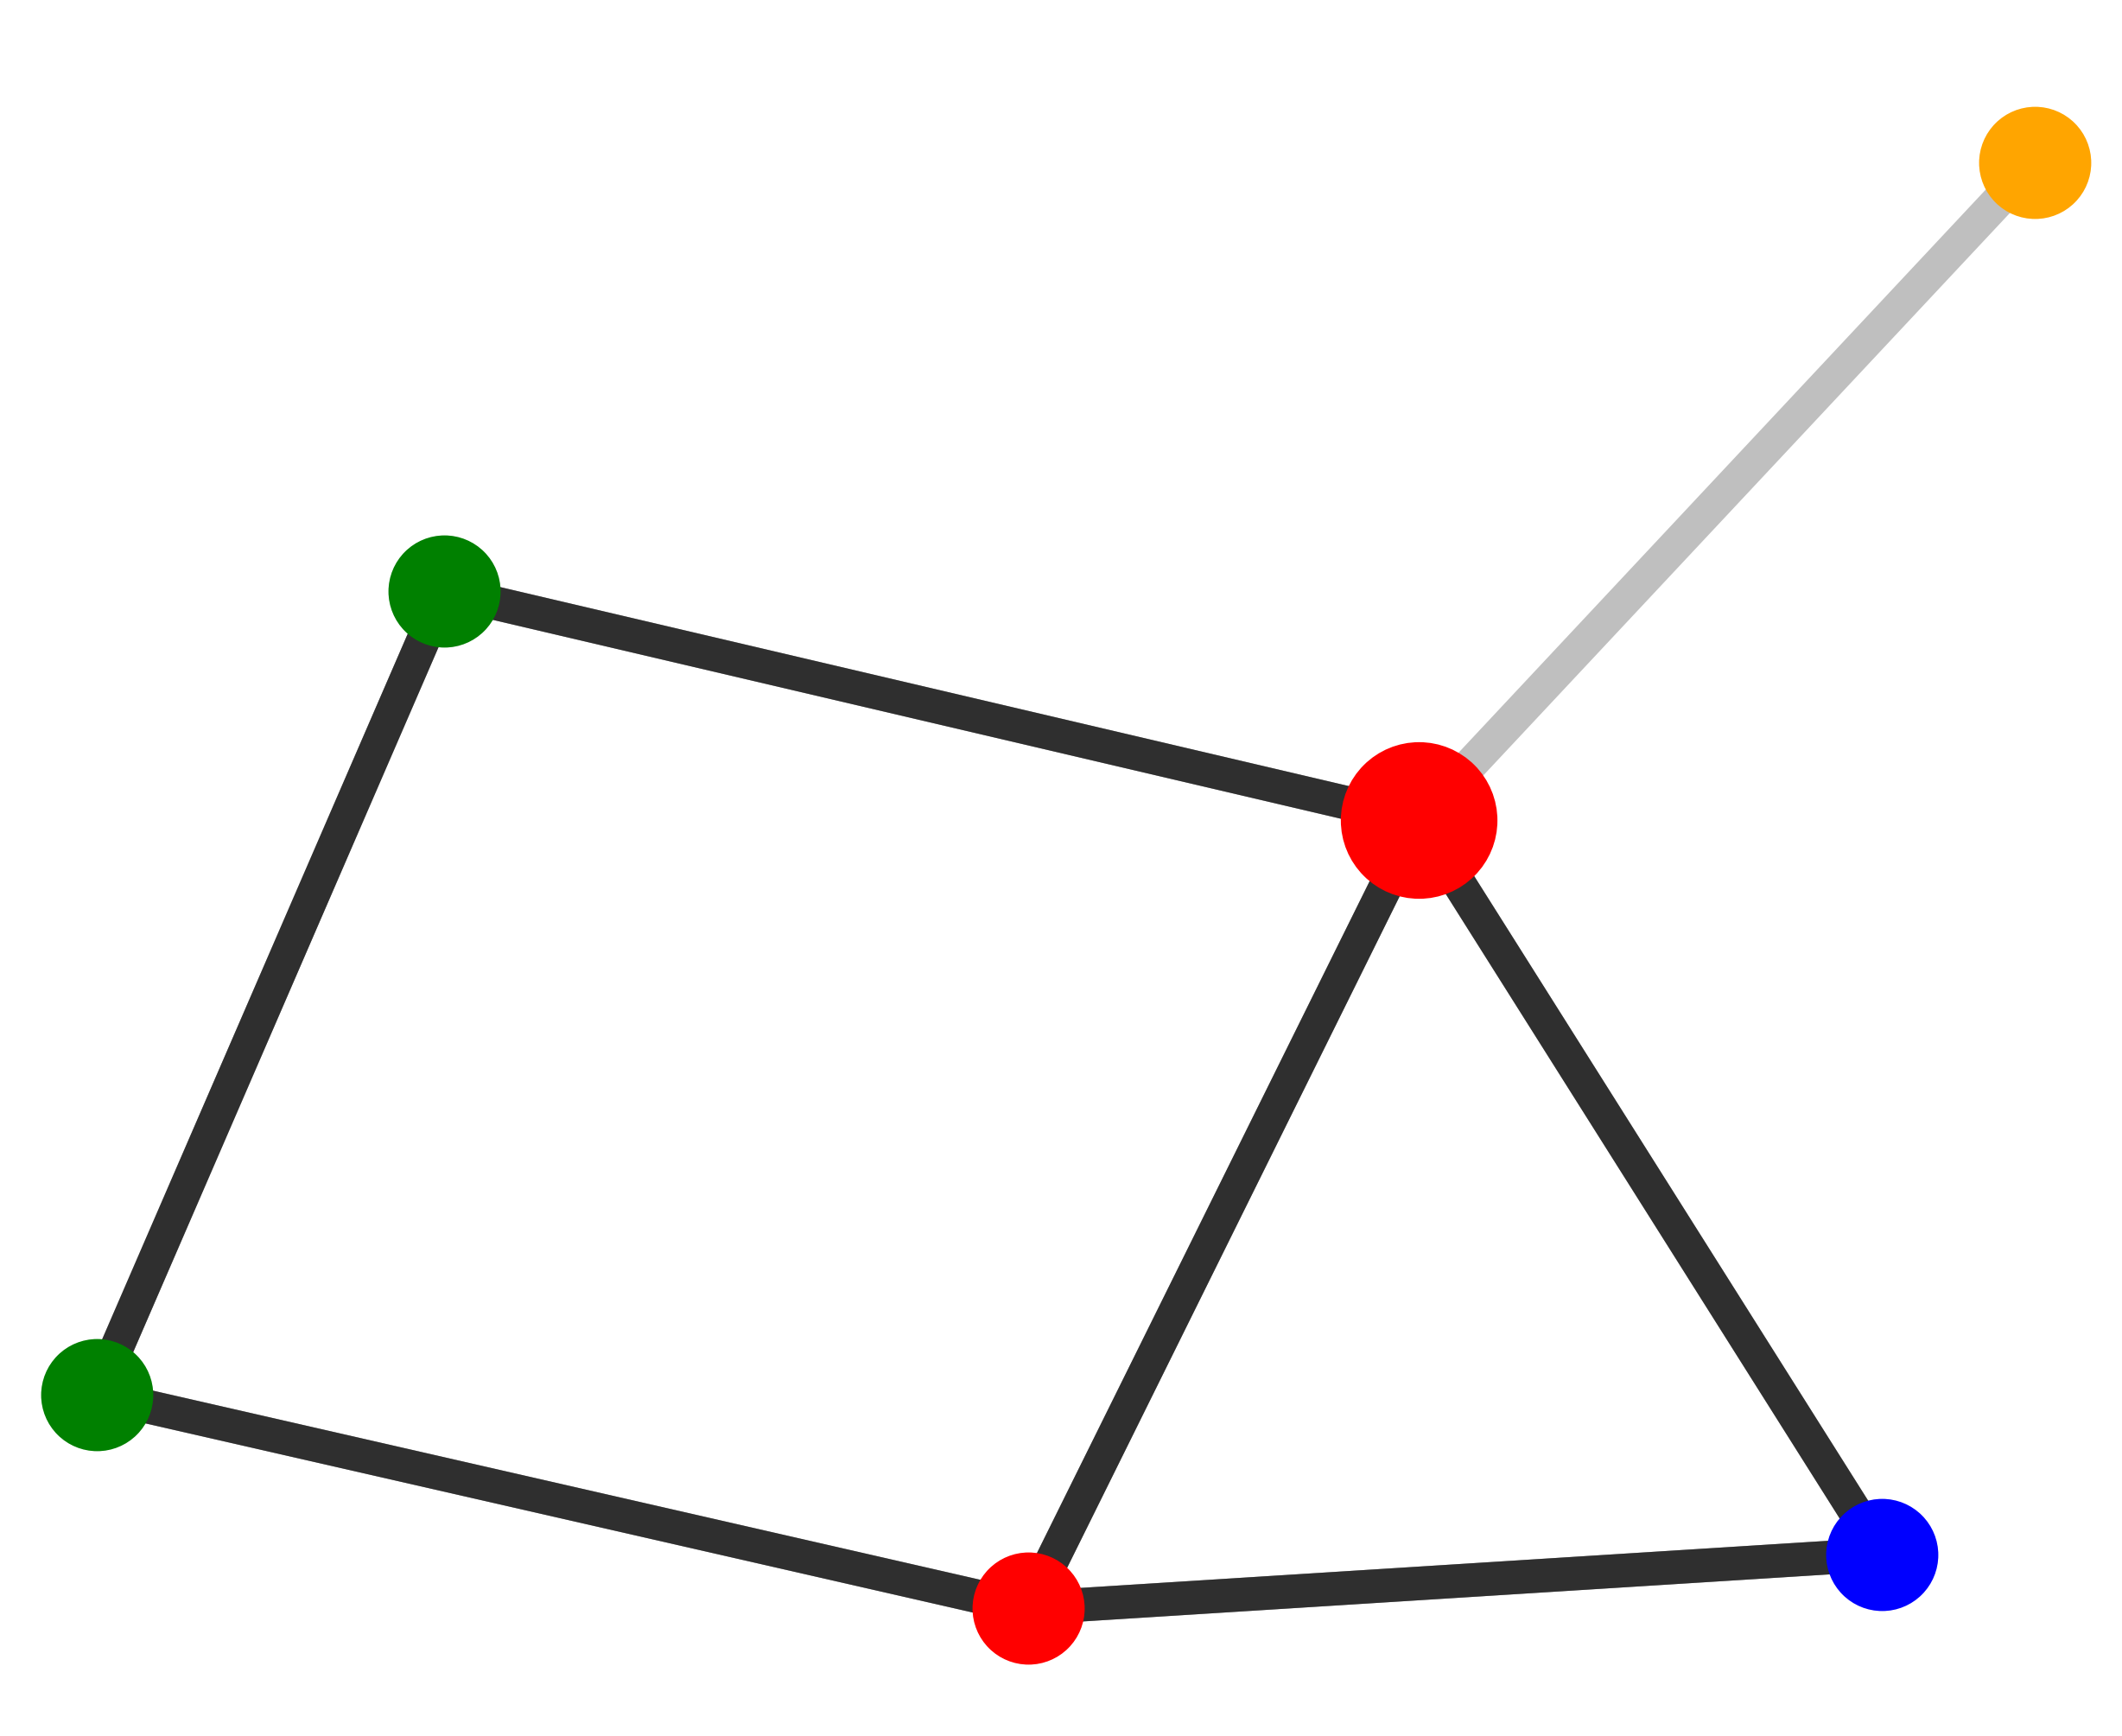
\includegraphics[width=.1\linewidth]{imgs/their_image-1.png}
% & 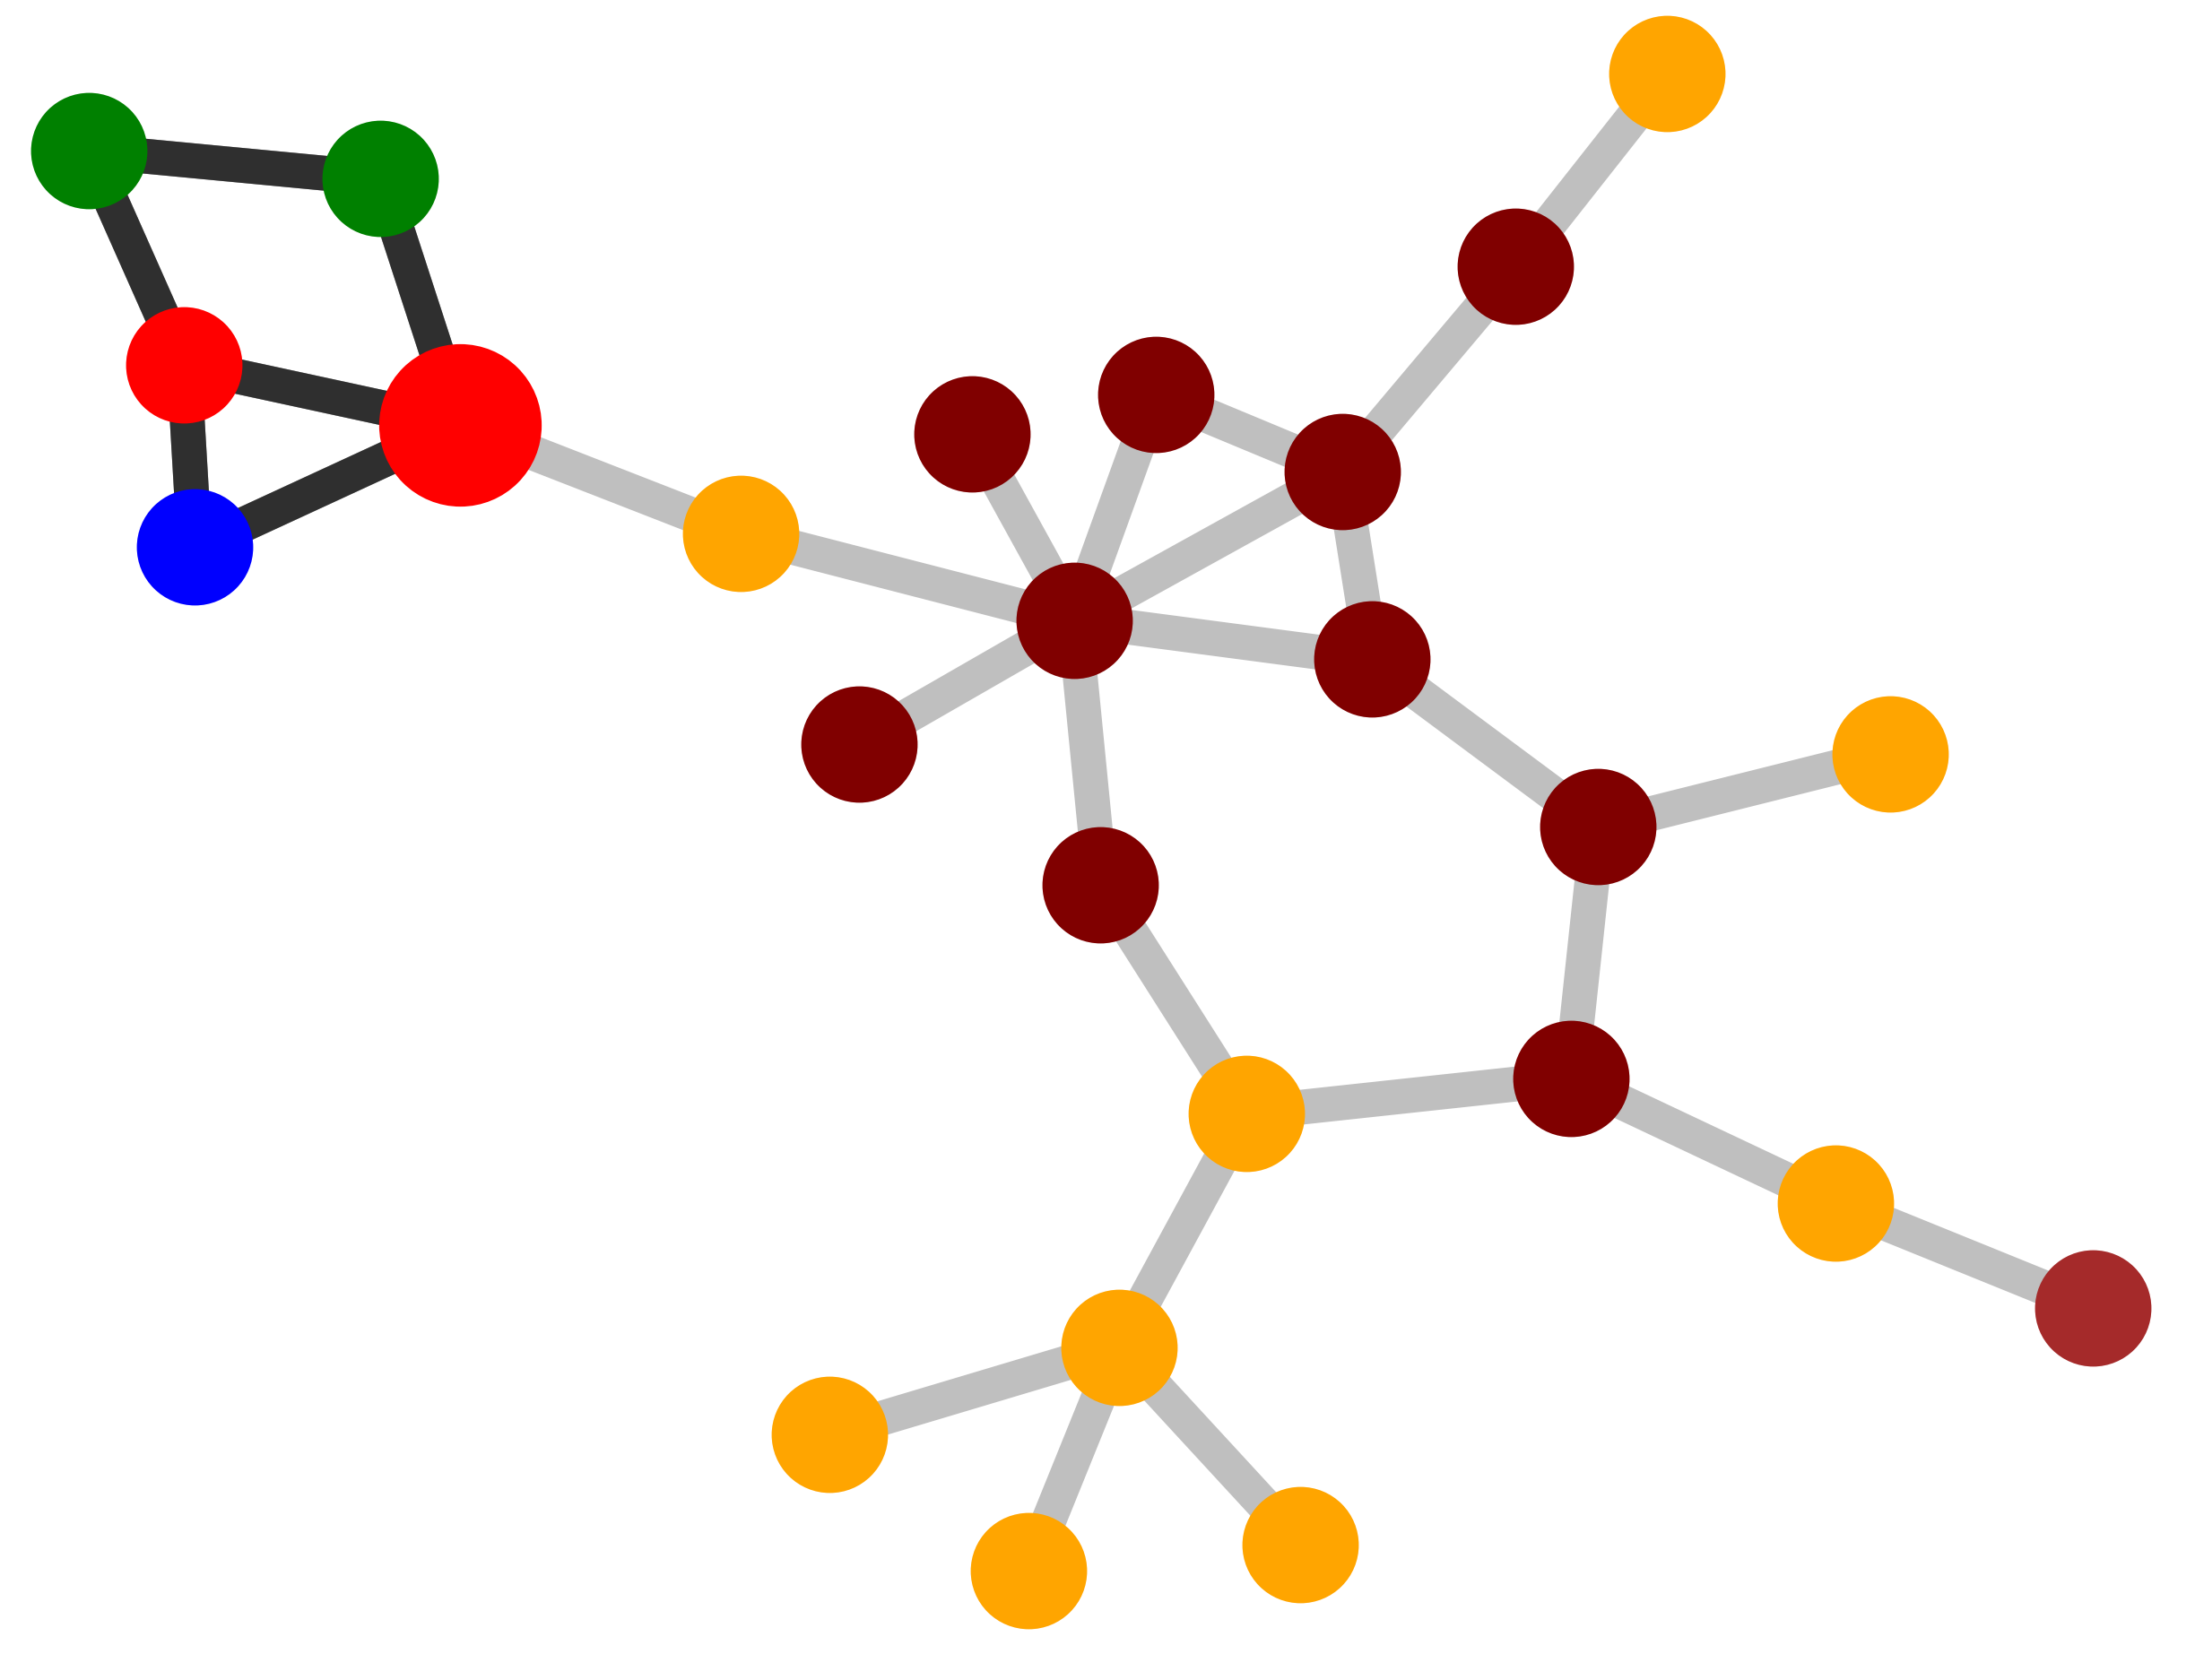
\includegraphics[width=.1\linewidth]{imgs/their_image-2.png} & 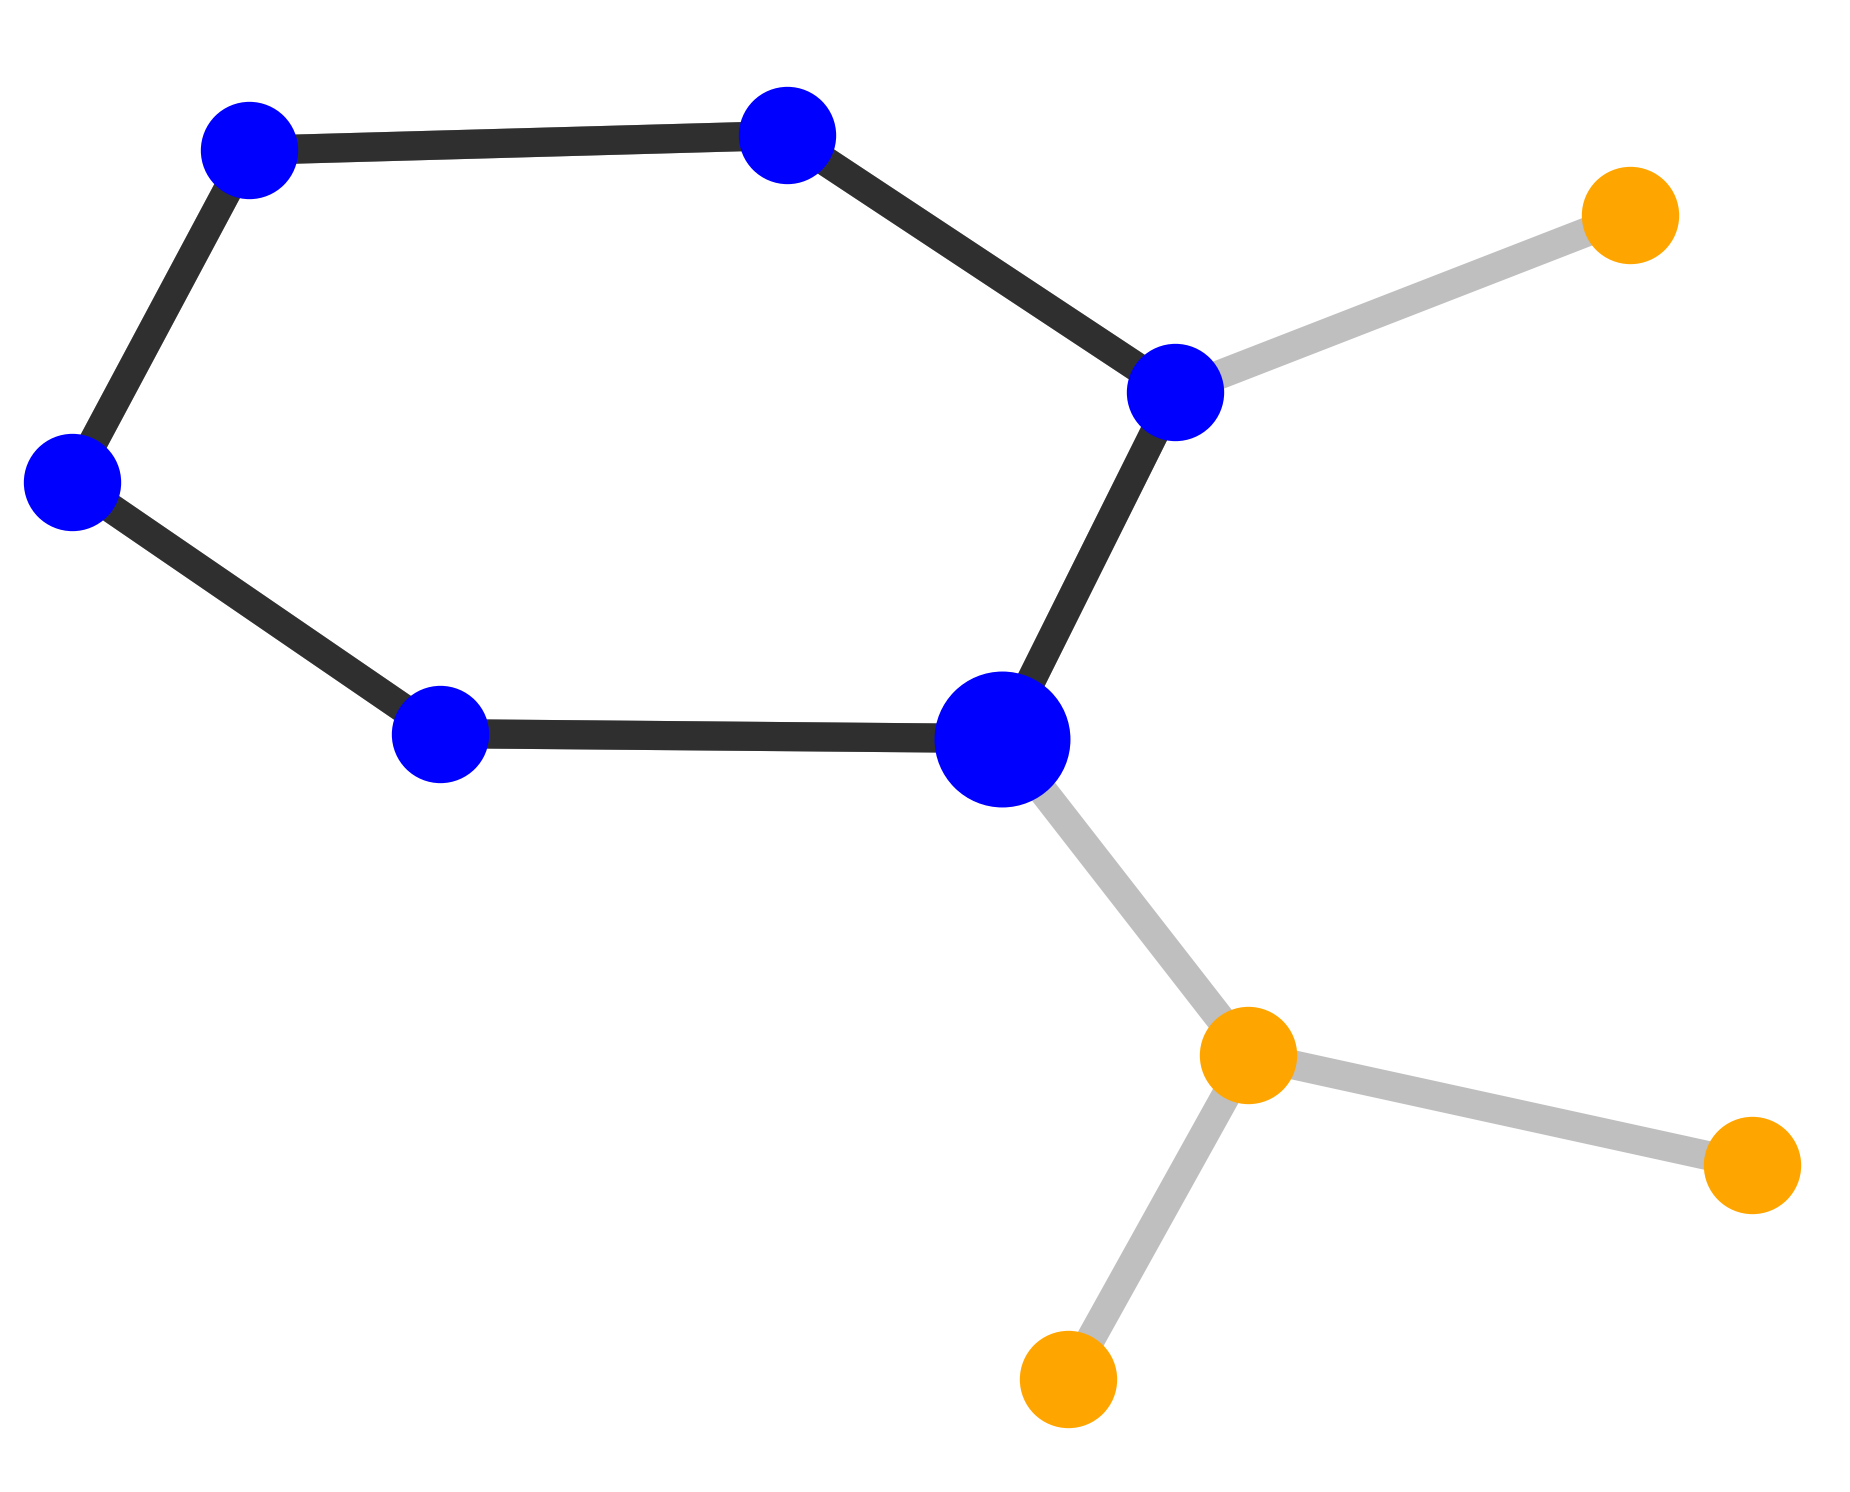
\includegraphics[width=.1\linewidth]{imgs/their_image-3.png} & \multicolumn{1}{l|}{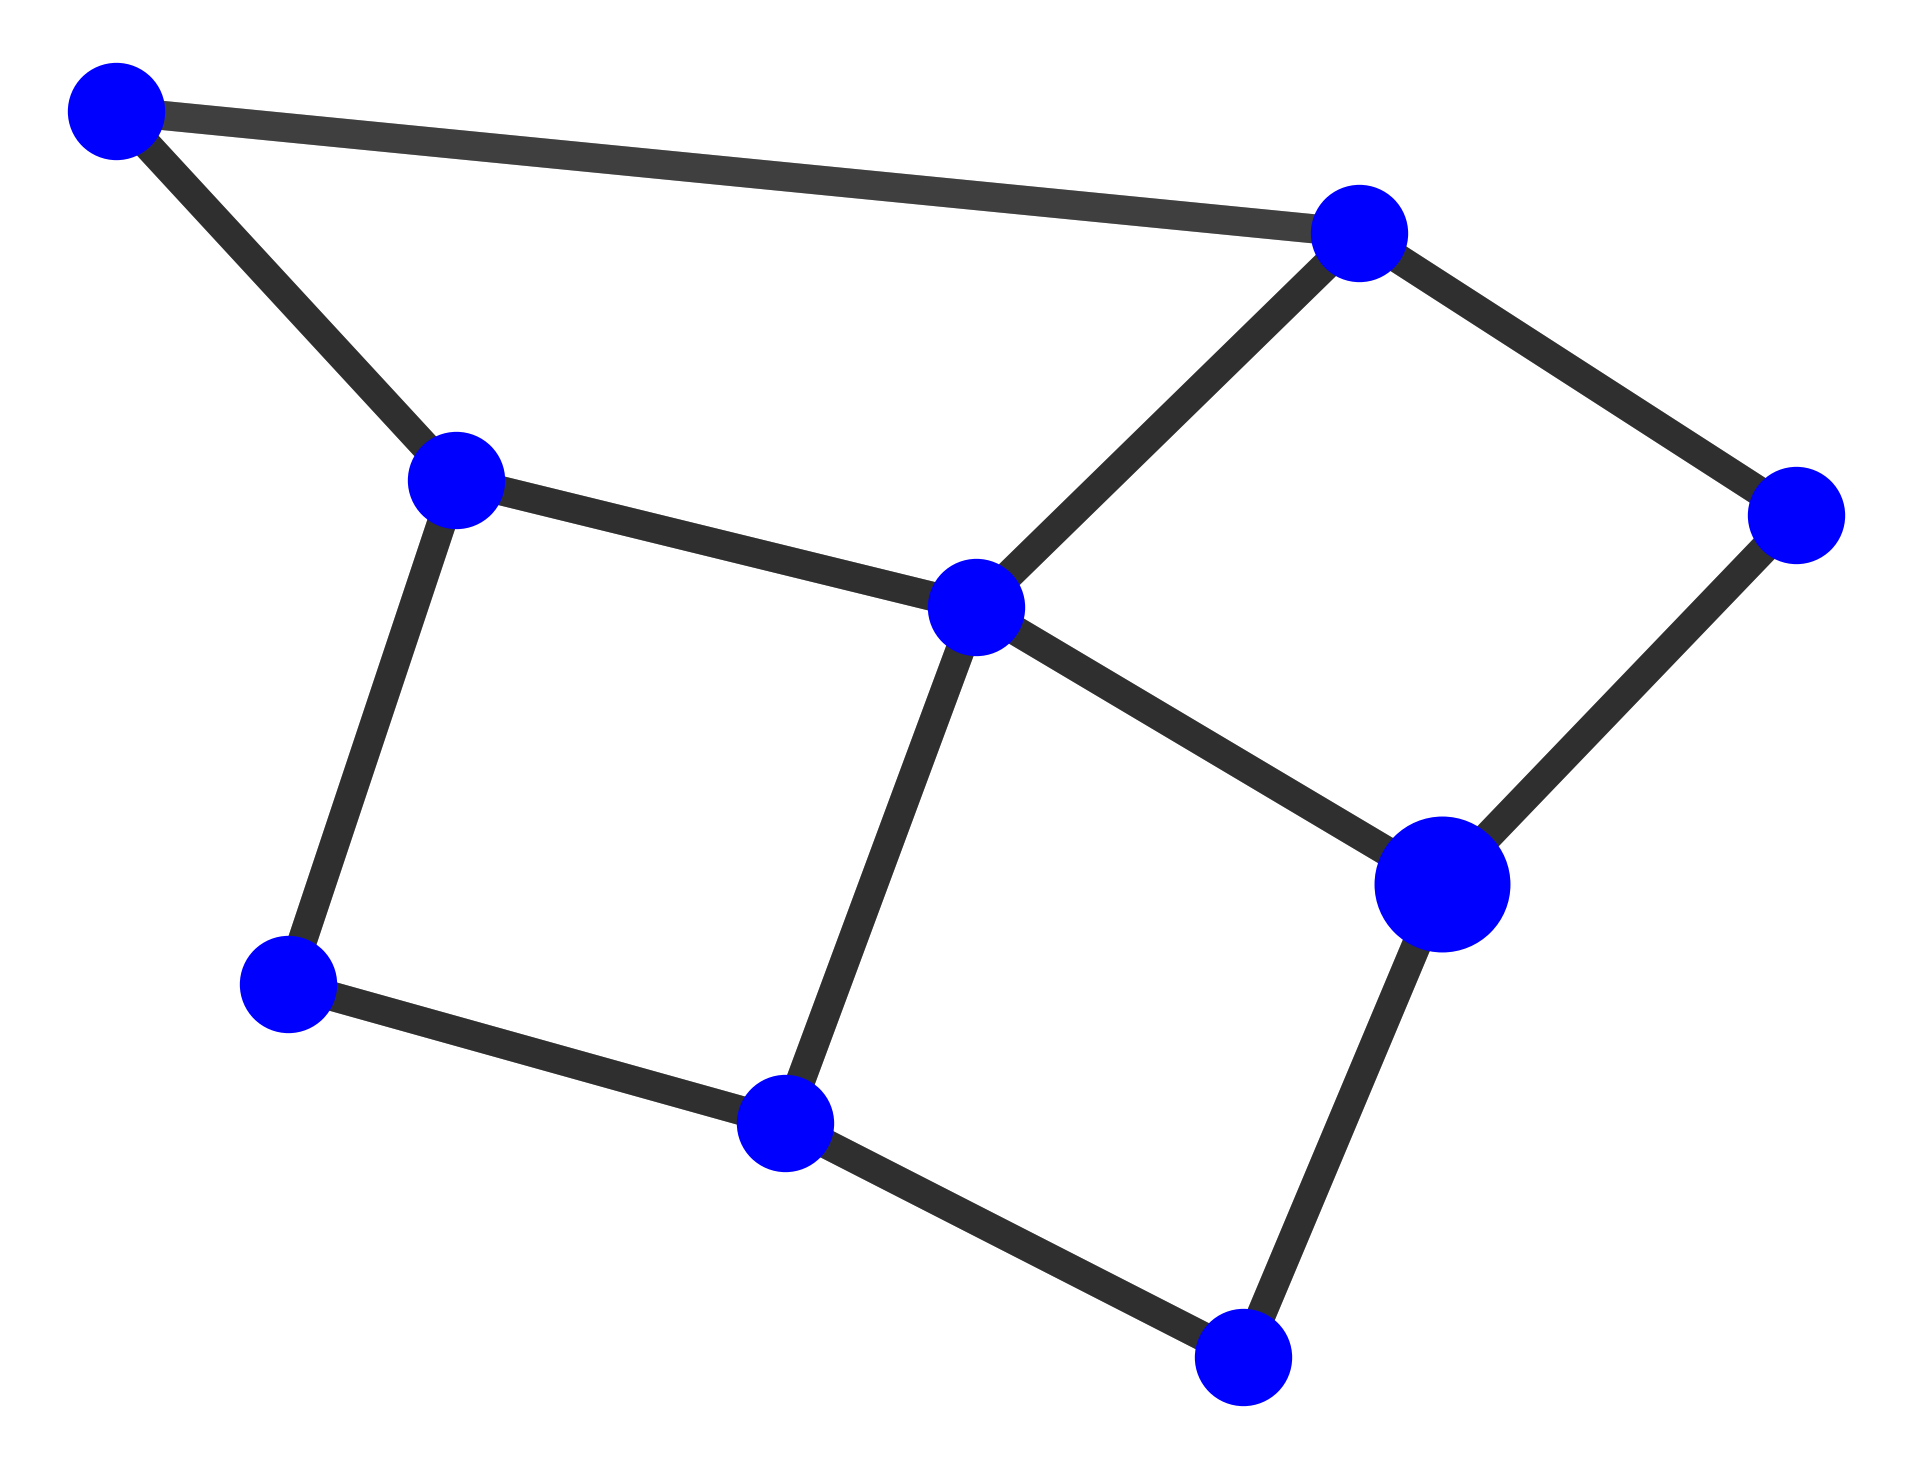
\includegraphics[width=.1\linewidth]{imgs/their_image-4.png}} & 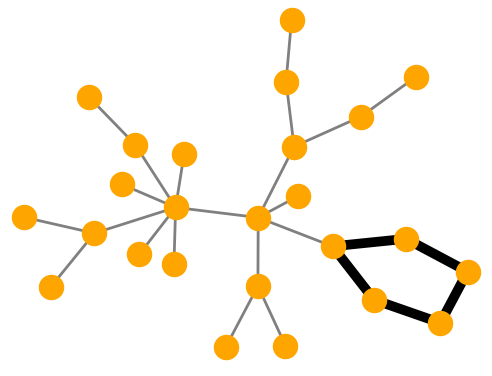
\includegraphics[width=.1\linewidth]{imgs/their_image-5.png} & 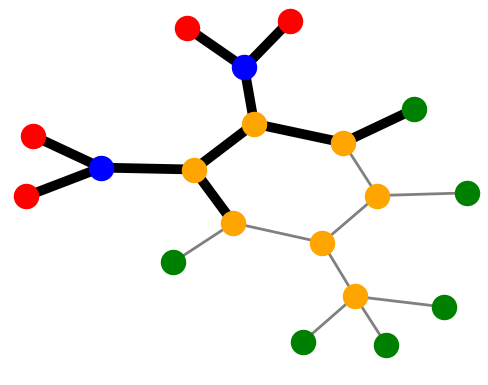
\includegraphics[width=.1\linewidth]{imgs/their_image-6.png} \\
% Reproduced & 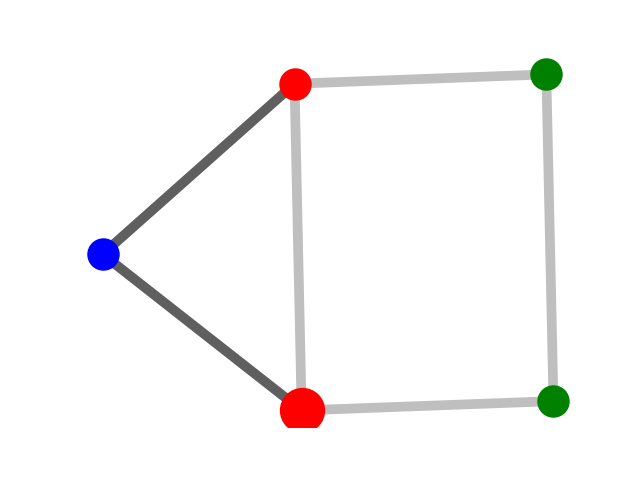
\includegraphics[width=.1\linewidth]{imgs/replication/syn1.png}
% & 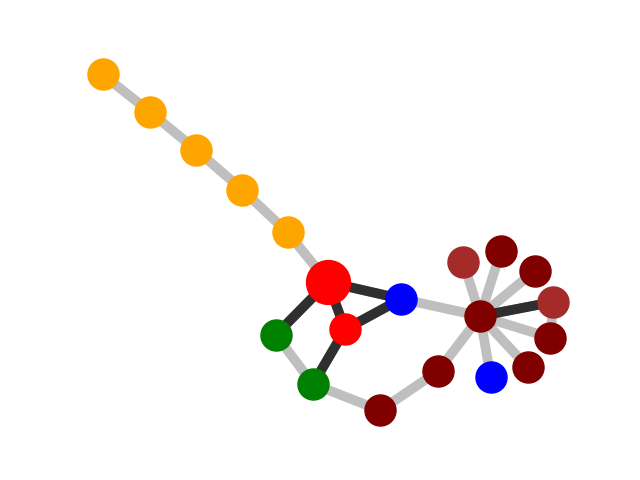
\includegraphics[width=.1\linewidth]{imgs/replication/syn2.png} & 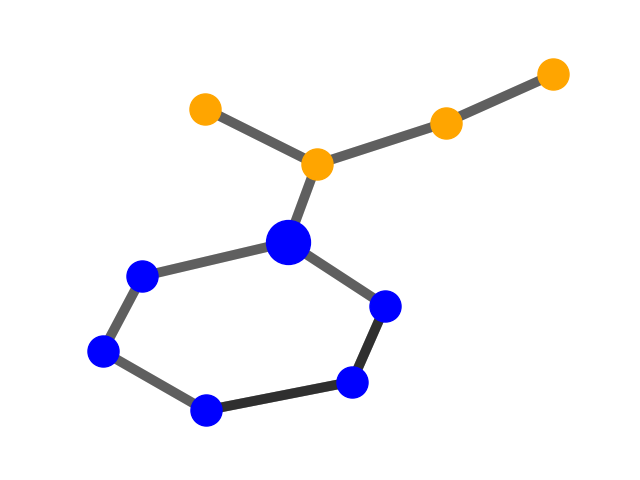
\includegraphics[width=.1\linewidth]{imgs/replication/syn3.png} & \multicolumn{1}{l|}{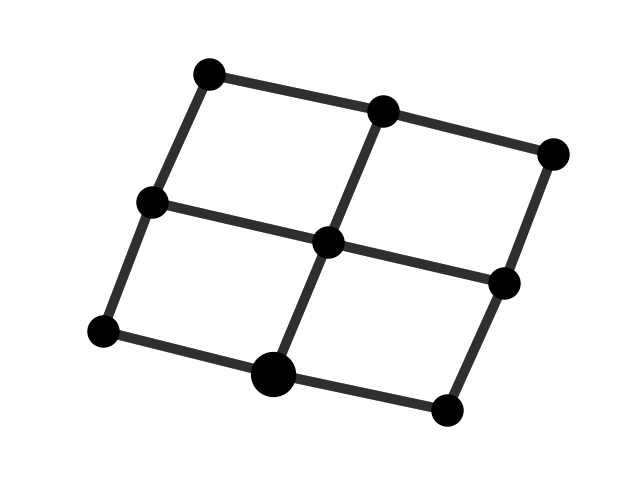
\includegraphics[width=.1\linewidth]{imgs/replication/syn4.png}} & img & 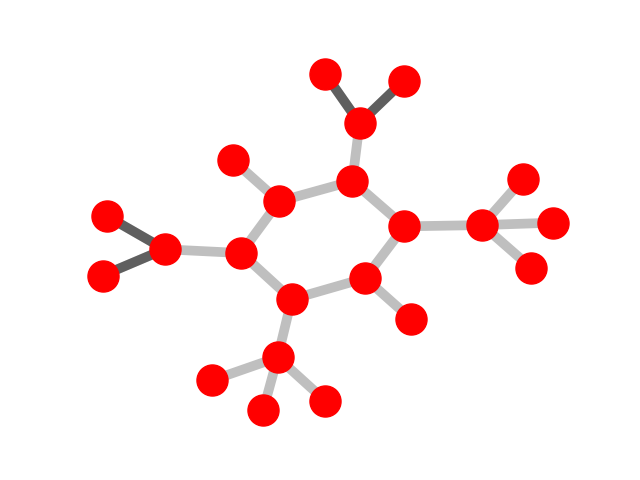
\includegraphics[width=.1\linewidth]{imgs/replication/85.png} \\ \hline
% \multicolumn{7}{l}{\textbf{Explanation AUC}} \\ \hline
% Original & 0.963 ± 0.011 & 0.945 ± 0.019 & 0.987 ± 0.007 & \multicolumn{1}{l|}{0.907 ± 0.014} & 0.926 ± 0.021 & 0.873 ± 0.013 \\ \hline
% Reproduced & 0.977 ± 0.006 & 0.970 ± 0.006 & 0.534 ± 0.186 & \multicolumn{1}{l|}{0.649 ± 0.045} & x.xx & 0.843 ± 0.084 \\ \hline
% \multicolumn{7}{l}{\textbf{Inference Time (ms)}} \\ \hline
% Reproduced & 3.56 & 5.29 & 0.40 & \multicolumn{1}{l|}{0.47} & x.xx & 2.09 \\ \bottomrule
% \end{tabular}
% \caption{Reproduction results}
% \label{tab:reproduction_results}
% \end{table}

% \paragraph{Qualitative}
% The replicated qualitative evaluation is very similar to the original results. PGExplainer is very capable of finding the motifs in the graphs and highlighting their edges. 

% \paragraph{Quantitative}
% The replicated quantitative evaluation shows results that are significantly different from the originals. Interestingly, the difference occurs in a different dataset then where the difference was observed in model accuracy. Despite the difference in validation and test accuracy between the replicated and the original model that is explained, the AUC score of the PGExplainer is very similar. On the other hand, the replicated evaluation of the tree-based graphs scores significantly lower, despite having very sensible qualitative explanations. One potential reason for this is the entropy and size regularization used in the PGExplainer. The configuration provided by the original codebase differ from the other datasets significantly for the tree-based datasets.

% \paragraph{Efficiency}
% Despite being evaluated using a considerably less powerful machine, and without utilizing a GPU, our implementation greatly outperforms the original implementation. 

% \subsection{Discussion}
% Based on the paper alone it is impossible to replicate the results presented in the paper, even if the complications of the evaluation itself are ignored. However, as the results presented above show, even with the provided codebase replicating the presented results is still not possible. First, the code base is badly structured and does not contain a central place describing the used configurations for training the models. Because of this a number of things remained unclear about the configuration of the models that might have lead to the reduced accuracy. For example, the training script configuration contained the possibility to use weight sharing and dropout to prevent over-fitting, but this is not used in any of the models. We hypothesize that this might be used for improving the accuracy of the BA-community model. 

% The replicated quantitative, qualitative and efficiency experiments similarly show that it is hard to reproduce the results prevented in the paper. Again, the main configuration files required to faithfully replicate the main results are missing. We believe that this effect is worsened by the crucial role of badly documented hyper parameters such as the entropy and size regularization coefficients. In the qualitative evaluation we expect that the importance of these hyper-parameters is hidden by the handpicked number of edges show in the explanation. The effect of these parameters will be further explored in the extended reproduction.


\section{Results}\label{sec:results}

\subsection{Model training \hfill \texttt{[experiment\_models\_training.ipynb]}}
\begin{table}[]
\centering
\begin{tabular}{cccccccc}
\toprule
&\multicolumn{4}{c}{\textbf{Node Classification}} & \multicolumn{2}{c}{\textbf{Graph Classification}} \\
Accuracy & \multicolumn{1}{c}{BA-Shapes} & \multicolumn{1}{c}{BA-Community} & \multicolumn{1}{c}{Tree-Cycles} & \multicolumn{1}{c|}{Tree-Grid} & \multicolumn{1}{c}{BA-2motifs} & \multicolumn{1}{c}{Mutagenicity} \\ 
\midrule
Training & 0.97 & 0.90 & 0.94 & \multicolumn{1}{c|}{0.96} & 1.00 & 0.82 \\
Validation & 1.00 & 0.75 & 0.98 & \multicolumn{1}{c|}{0.99} & 1.00 & 0.82 \\
Testing & 1.00 & 0.72 & 0.94 & \multicolumn{1}{c|}{0.99} & 0.99 & 0.81 \\
\bottomrule
\end{tabular}
\caption{Accuracies of the trained model without batch-normalization. The accuracies are obtained using early stopping. }
\label{tab:simp_accs}
\end{table}
In Tab.~\ref{tab:simp_accs} the final accuracies for all 6 trained models are provided. Note that these are the accuracies of the models that will be explained by the two explainers, not the explanation accuracy of the explainers themselves. For most of the models, using the configurations found in the code, we achieve results comparable to the results presented in the paper. The two exceptions being the BA-Community and the Mutagenicity models. Both of these score lower then their original counterpart. 

Logically this difference could be contributed to the difference in the use of batch normalization. Where the original model in the PGExplainer paper did use batch normalization where we do not. However, as the results presented in Tab.\,\ref{tab:accuracies} show, replication with the original batch normalization yields the same reduced accuracies. We hypothesise that therefore the difference might be the result of an undocumented use of weight regularization. We observed that in the original training script the configuration exist to use L2-weight regularization, but it is not used.

\subsubsection{Replicability study \hfill \texttt{[experiment\_replication.ipynb]}}
\paragraph{Quantitative}
\begin{table}[h!]
\centering
\scalebox{0.95}{
\begin{tabular}{rcccccc}
\toprule
\multicolumn{5}{c}{\textbf{Node Classification}} & \multicolumn{2}{c}{\textbf{Graph Classification}} \\
\multicolumn{1}{c}{} & \multicolumn{1}{c}{BA-Shapes} & \multicolumn{1}{c}{BA-Community} & \multicolumn{1}{c}{Tree-Cycles} & \multicolumn{1}{c|}{Tree-Grid} & \multicolumn{1}{c}{BA-2motifs} & \multicolumn{1}{c}{Mutagenicity} \\ \hline
\multicolumn{7}{l}{\textbf{Visualization (qualitative)}} \\ \hline
PGExplainer &  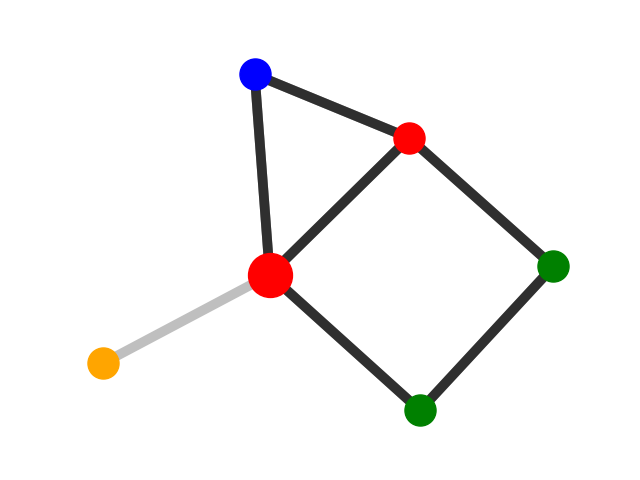
\includegraphics[width=.1\linewidth]{../openreview/imgs/simplification/syn1_pg.png}
& 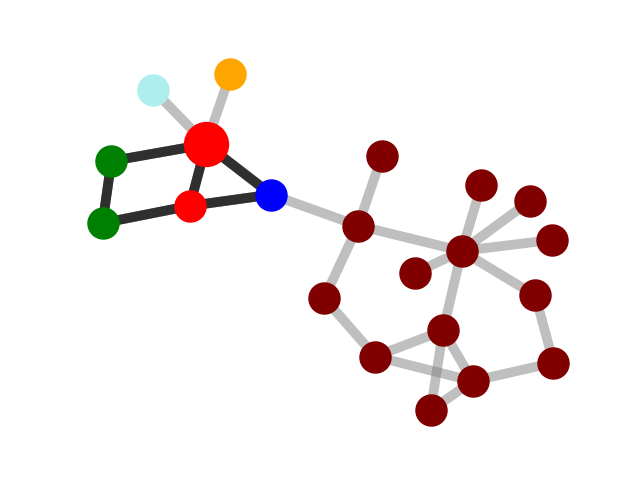
\includegraphics[width=.1\linewidth]{../openreview/imgs/simplification/syn2_pg.png} & 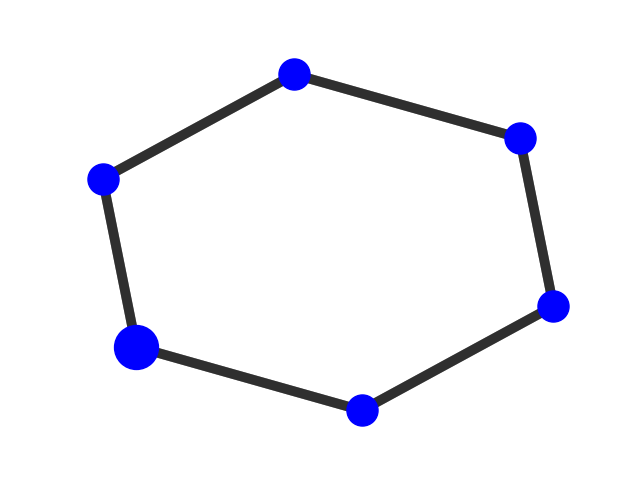
\includegraphics[width=.1\linewidth]{../openreview/imgs/simplification/syn3_pg.png} & \multicolumn{1}{l|}{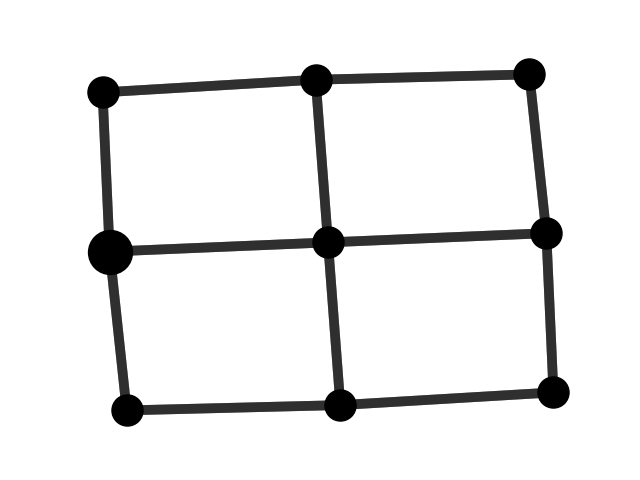
\includegraphics[width=.1\linewidth]{../openreview/imgs/simplification/syn4_pg.png}} & 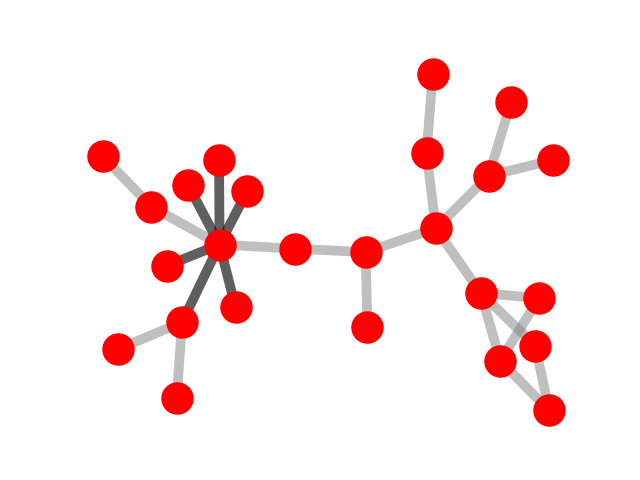
\includegraphics[width=.1\linewidth]{../openreview/imgs/simplification/ba_pg.png} & 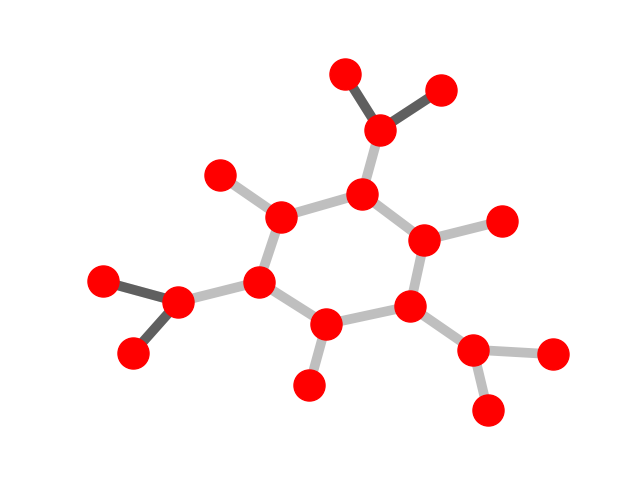
\includegraphics[width=.1\linewidth]{../openreview/imgs/simplification/mutag_pg.png} \\ \hline
% PGExplainer (bad) &  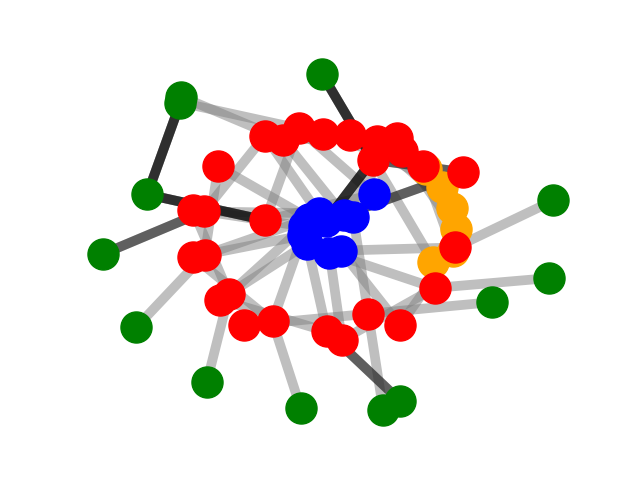
\includegraphics[width=.1\linewidth]{imgs/extension/pg/syn1_bad.png}
% & 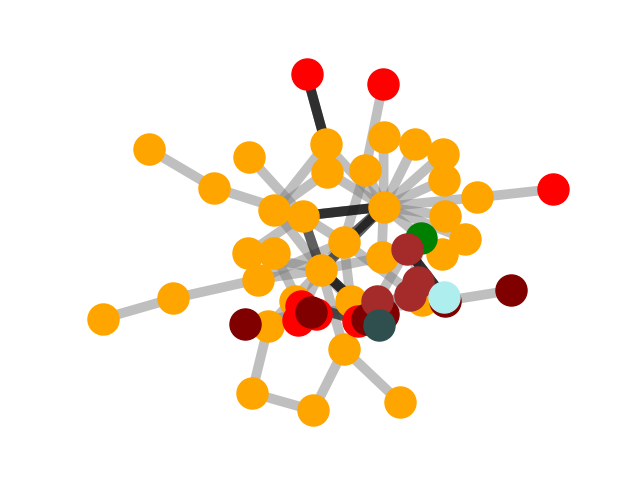
\includegraphics[width=.1\linewidth]{imgs/extension/pg/syn2_bad.png} & 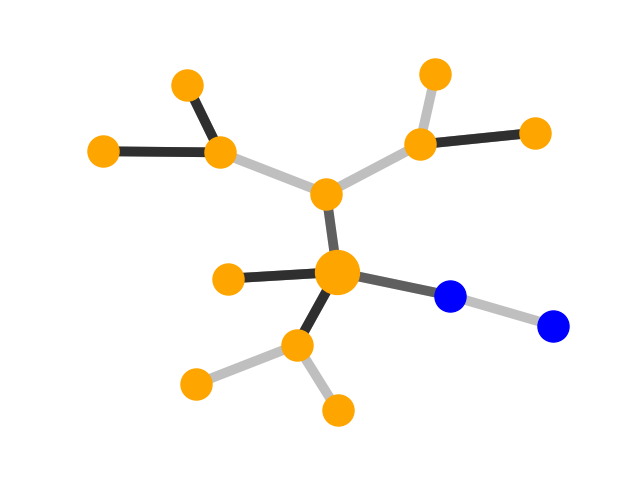
\includegraphics[width=.1\linewidth]{imgs/extension/pg/syn3_bad.png} & \multicolumn{1}{l|}{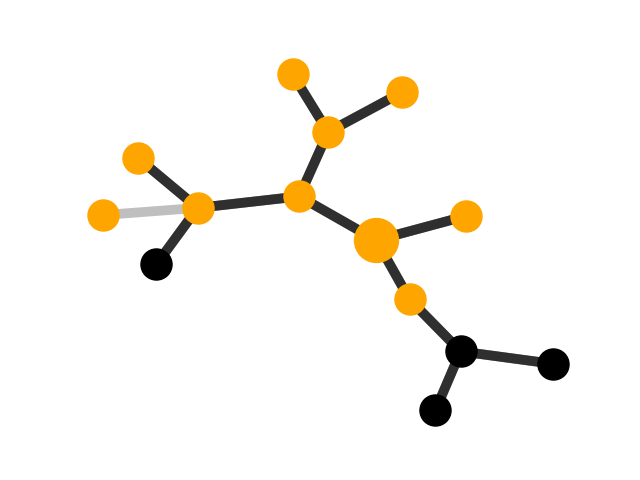
\includegraphics[width=.1\linewidth]{imgs/extension/pg/syn4_bad.png}} & \includegraphics[width=.1\linewidth]{imgs/-5.png} & 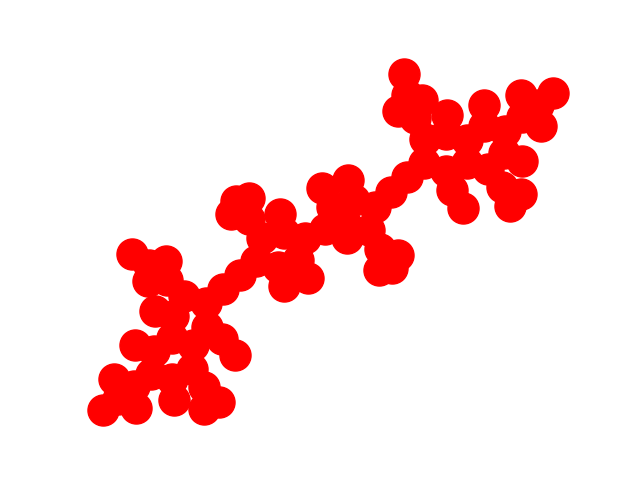
\includegraphics[width=.1\linewidth]{imgs/extension/gnn/mutag_bad.png} \\
GNNExplainer &  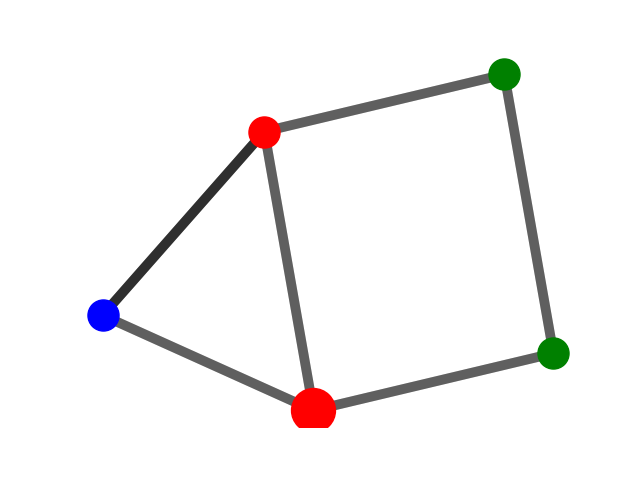
\includegraphics[width=.1\linewidth]{../openreview/imgs/simplification/syn1_gnn.png}
& 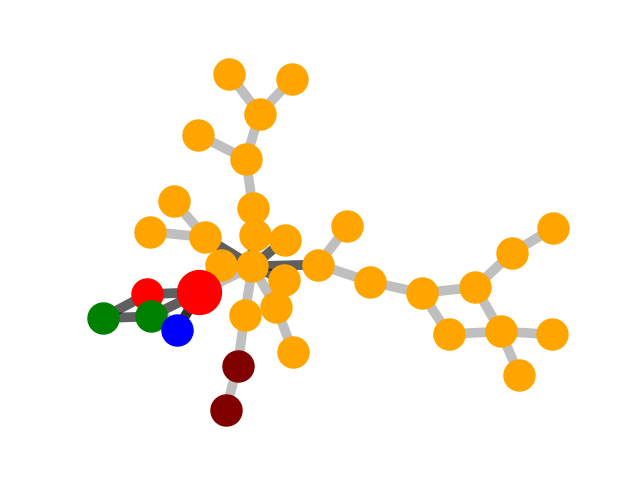
\includegraphics[width=.1\linewidth]{../openreview/imgs/simplification/syn2_gnn.png} & 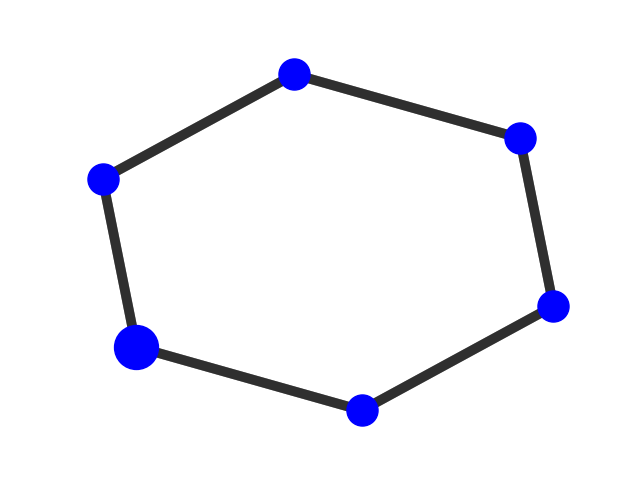
\includegraphics[width=.1\linewidth]{../openreview/imgs/simplification/syn3_gnn.png} & \multicolumn{1}{l|}{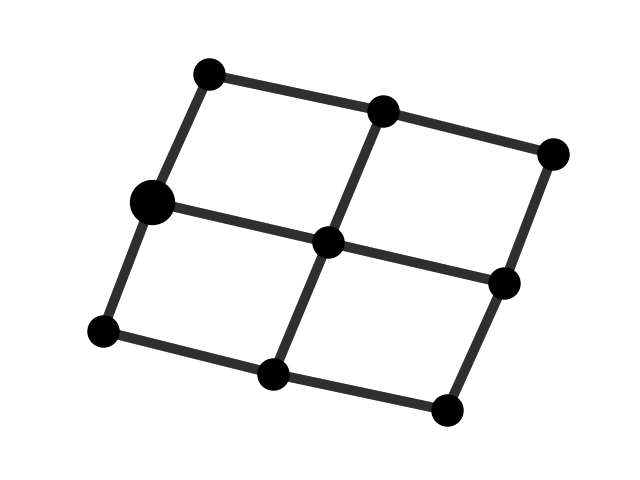
\includegraphics[width=.1\linewidth]{../openreview/imgs/simplification/syn4_gnn.png}} & 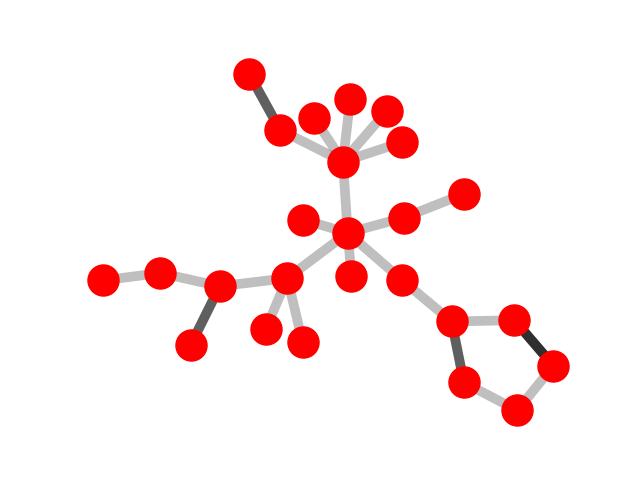
\includegraphics[width=.1\linewidth]{../openreview/imgs/simplification/ba_gnn.png} & 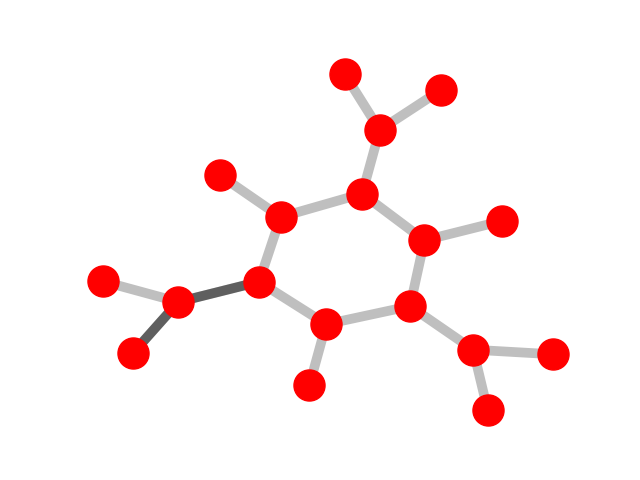
\includegraphics[width=.1\linewidth]{../openreview/imgs/simplification/mutag_gnn.png} \\\hline
% GNNExplainer (bad) &  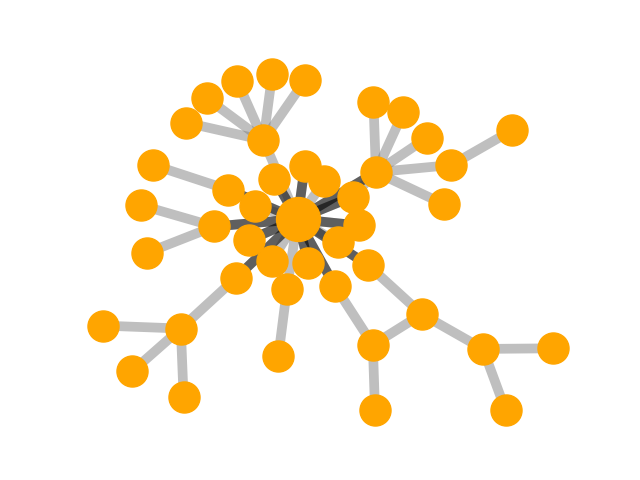
\includegraphics[width=.1\linewidth]{imgs/extension/gnn/syn1_bad.png}
% & 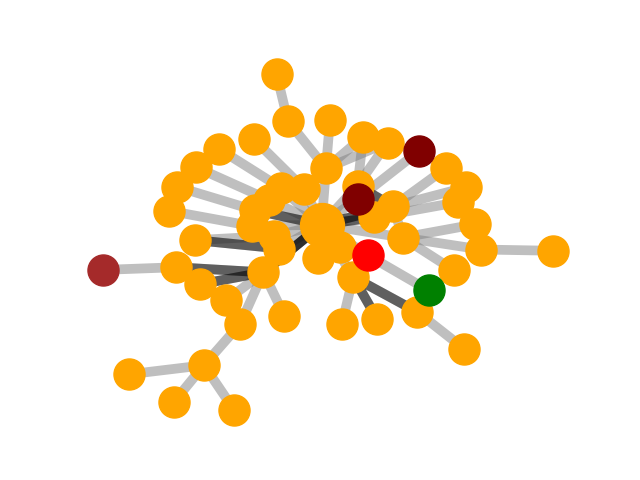
\includegraphics[width=.1\linewidth]{imgs/extension/gnn/syn2_bad.png} & 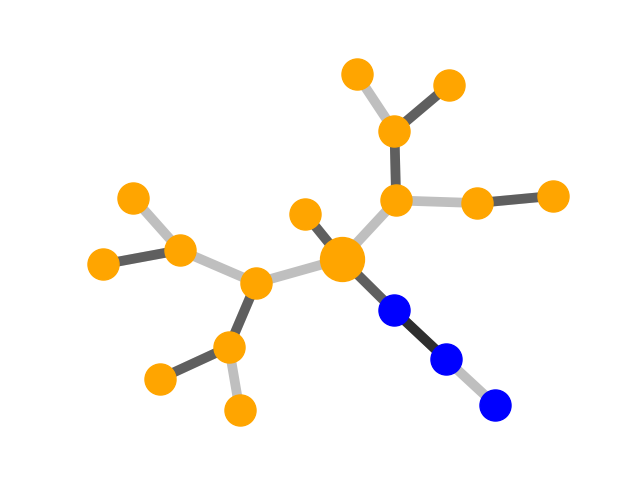
\includegraphics[width=.1\linewidth]{imgs/extension/gnn/syn3_bad.png} & \multicolumn{1}{l|}{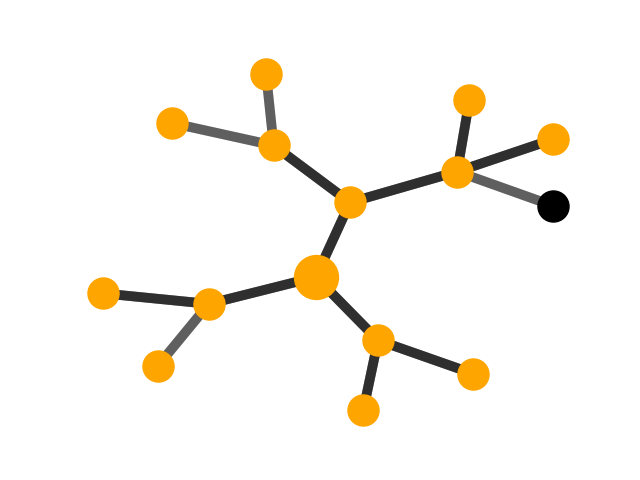
\includegraphics[width=.1\linewidth]{imgs/extension/gnn/syn4_bad.png}} & \includegraphics[width=.1\linewidth]{imgs/-5.png} & \includegraphics[width=.1\linewidth]{imgs/-6.png} \\\hline
\multicolumn{7}{l}{\textbf{Explanation AUC (quantitative}} \\ \hline
Original & 0.963 ± 0.011 & 0.945 ± 0.019 & 0.987 ± 0.007 & \multicolumn{1}{l|}{0.907 ± 0.014} & 0.926 ± 0.021 & 0.873 ± 0.013 \\ 
PGExplainer & 0.999 ± 0.000 & 0.825 ± 0.040 & 0.760 ± 0.014 & \multicolumn{1}{l|}{0.679 ± 0.008} & 0.133 ± 0.046 & 0.843 ± 0.084 \\ 
GNNExplainer & 0.742 ± 0.006 & 0.708 ± 0.004 & 0.540 ± 0.017 & \multicolumn{1}{l|}{0.714 ± 0.002} & 0.499 ± 0.004 & 0.587 ± 0.002 \\ 
Improvement & 34.6\% & 16.5\% & 40.7\% & \multicolumn{1}{l|}{-4.9\%} & -375.2\% & 43.6\% \\ \hline
\multicolumn{7}{l}{\textbf{Inference Time (ms) (efficiency)}} \\ \hline
PGExplainer & 3.58 & 5.23 & 0.45 & \multicolumn{1}{l|}{0.54} & 0.33 & 2.05 \\
GNNExplainer & 58.80 & 91.81 & 52.81 & \multicolumn{1}{l|}{65.54} & 5.21 & 12.32 \\
Speedup & 16x & 17x & 117x & \multicolumn{1}{l|}{121x} & 16x & 6x \\
\bottomrule
\end{tabular}}
\caption{Replicated experimental results from the quantitative, qualitative and efficiency study. The original scores are copied from the paper directly. As the authors of the PGExplainer paper did not report the seeds used for the 10 validation results, we were unable to replicate these results using the authors own codebase. For the qualitative visualization the samples are handpicked similar to the original paper. Node colors represent the node labels (if all colours are the same the nodes are unlabeled). Darkness of the edges signals importance for the final classification decision. In case of the node-classification datasets the bigger node is the one for which the classification is being explained. For the quantitative explanation the average AUC score for the PGExplainer and GNNExplainer and the standard deviation is given. The "original" row reports the PGExplainer AUC score from the original paper. The inference time reported represents the time needed to explain a single sample in milliseconds.}
\label{tab:reproduction_results2}
\end{table}

Quantitatively there is a large difference in the reported AUC scores and what we were able to achieve using the specified configurations for the PGExplainer. Only for BA-Shapes a AUC equal or higher then the presented AUC score was observed. However, BA-Shapes did require some minor modifications to the configurations to get it to work. With the temperature parameter set as originally presented in the code, the evaluation crashed. Only when the temperature was changed to the configuration as presented in the paper we were able to run the evaluation. Similarly, with the configuration as described in the code, the PGExplainer produces the opposite of the expected result for the BA-2Motifs dataset. This is reflected both quantitatively and qualitatively. However, it should be noted that the same drop in AUC score between our implementation and the one originally reported score can also be seen for the GNNExplainer. Due to this, the reported improvement of the PGExplainer over the GNNExplainer remains valid. 

We believe that the difference seen between the AUC scores originally reported for the two explainers and what we observed during our reproduction might be the result of the undocumented effect of the entropy/size regularizations and used temperature. Based on empirical observations we found that the final AUC score is highly dependent on these three hyperparameters. A small follow-up ablation study presented in Tab.\,\ref{tab:reg} confirms this. 

\begin{table}[]
\scalebox{0.97}{
\begin{tabular}{@{}c|l|llllll@{}}
\toprule
\multicolumn{1}{l|}{\textbf{Reg.}} &       & \multicolumn{6}{c}{\textbf{Size}}                                                                \\ \midrule
\multicolumn{1}{l|}{}              &       & 10            & 1             & 0.1           & 0.01        & 0.001       & 0.0001               \\ \midrule
\multirow{5}{*}{\textbf{Entropy}}  & 10    & 0.761 ± 0.014 & 0.761 ± 0.014 & 0.762 ± 0.014 & 0.713 ± 0.156 & 0.628 ± 0.221 & 0.634 ± 0.239          \\
                                  & 1     & 0.761 ± 0.014 & 0.760 ± 0.014   & 0.760 ± 0.015   & 0.683 ± 0.154 & 0.700 ± 0.247 & 0.708 ± 0.226          \\
                                  & 0.1   & 0.761 ± 0.014   & 0.760 ± 0.014   & 0.758 ± 0.015   & 0.565 ± 0.246 & 0.747 ± 0.209 & 0.764 ± 0.214          \\
                                  & 0.01  & 0.761 ± 0.014   & 0.760 ± 0.014   & 0.758 ± 0.015   & 0.551 ± 0.249 & 0.748 ± 0.216 & \textbf{0.776 ± 0.210} \\
                                  & 0.001 & 0.761 ± 0.014   & 0.760 ± 0.014   & 0.758 ± 0.015   & 0.547 ± 0.253 & 0.753 ± 0.216 & 0.763 ± 0.211          \\ \bottomrule
\end{tabular}
}
\label{tab:reg}
\caption{Results of a small ablation study on the effect of the size and entropy regularization on the AUC score. The ablation study is performed using the Tree-Cycles dataset and follows the setup of the quantitative evaluation. It averages over 10 runs. The results show that the regularization has a large effect on both the quantitative quality of the explanations and their consistency. The best score is shown in bold. \hfill \texttt{[experiment\_ablation.ipynb]}}
\end{table}

\paragraph{Qualitative}
The replicated qualitative evaluation is very similar to the original results. PGExplainer is very capable of finding the motifs in the graphs and highlighting their edges. The same holds for the GNNExplainer. 

The main observed difference is the Mutagenicity dataset. In our replication, only two edges are darkened in contrast to the ten edges darkened in the original paper. However, this difference is created artificially by a difference in the $k$ value reported in the paper and used in the code. While this difference therefore does not tell us anything about the quality of the explanation, it does show the importance of the $k$ hyperparameter. This is further discussed in the Sec.\,\ref{sec6}.

\paragraph{Efficiency}
In terms of efficiency, the reimplemention results are consistent with the claims of the authors. The use of different frameworks between the original implementation and our reimplementation makes a direct comparison of the result is ill advised, but the speedup between the PGExplainer and the GNNExplainer is consistent.
\section{Ground truth explanations for Graph Explanations} \label{sec6}
For the evaluation of the PGExplainer the authors made use of predefined ground-truth explanations. These explanations are made possible by the use of synthetic datasets, generated based on the notion of motifs. In this section we express some concerns with regards to the use of motifs for generating ground-truth explanations. 

\paragraph{No ground-truth outside motif}
In the case of the node classification datasets the definition of the ground-truth explanation is only valid for a small number of nodes within a graph; those within a motif. In essence, for nodes outside the motifs, the ground-truth explanation is an empty graph---i.e. all surrounding edges have to be excluded from the explanation to achieve the maximum score. The same is true for non-mutagenic graphs in the Mutagenicity dataset. This is incompatible with the PGExplainers approach to determine its explanation. An empty graph can never produce the same explanation as the original graph, hence it will never be the explanation provided by the PGExplainer. 

The authors overcome this issue by excluding all nodes outside the motifs from their quantitative evaluation. However, this reduces the explanation task of the node classification datasets to a much simpler problem. For nodes outside the motif, the explanation has to be based on the absence instead of presence of edges. Solving these issues satisfactorily would require a new definition for the ground-truths for graph datasets. For example, in the case of the tree-cycle dataset, one could define the ground-truth of a node outside a motif to be the entire 7-hop subgraph as this would be the minimal number of steps to take before one can conclude that no cycles have been formed. We, however, believe this to be outside the scope of this replication.


\paragraph{Qualitative evaluation dependent on knowing size of motif}
The PGExplainer gives as output a mask that describes for each edge in the graph the probability of it being important for the models classification decision. To turn this into a visualizable explanations the top-$k$ edges are selected from each mask, i.e only the $k$ edges that have the highest influence on the models classification decision are considered part of the explanation. As a result, $k$ is a crucial hyperparameter for obtaining a visual explanation. If $k$ is set too high, the explanation could contain edges that actually only contribute to the final decision marginally. If $k$ is set too low, the explanation could be missing important parts of the graph. This difference in visual explanation quality was also empirically observed in the difference between the original and our explanations for the Mutagenicity dataset. 

As mentioned in the experimental setup of the qualitative evaluation, the authors, and preceding works, set the value of $k$ in the evaluation based on the amount of edges in the defining motif. However, this is not a possibility outside of the synthetic evaluation datasets. Hence, for real world applicability of the proposed explanation method a different approach has to be found to find $k$. For this reason, we believe that evaluating the quality of the explanations based using $k$ preset to the number of edges in the synthetic dataset is an aspect to reconsider. 

In essence, both the $k$-parameter and the earlier mentioned number of edges selected for the ground-truth can be considered as hyperparameters for the evaluation pipeline. By selecting a specific value for these parameters the evaluation can become biased towards assigning high credibility to explanations that have a specific characteristic. By performing an extensive search over these hyperparameters the results of the explanation evaluation can potentially be improved. In Sec.\,\ref{sec:extended_replication} of the appendix we present a short study on how these hyperparameters can influence the final results of the evaluation. 
\section{Conclusion}\label{sec:conclusion}
In this work, we have presented a replication of the paper \textit{Parameterized Explainer for Graph Neural Network}. The replication experiments have lead us to a number of conclusions. First, based on the paper alone, it is difficult to replicate the presented results. The main contributing factor is the discrepancy between the provided details in the paper and those in the codebase. Based on communication with the authors, we conclude that the hyperparameter settings presented in the paper are oversimplified. For the method to work, more hyperparameter tuning is needed then the paper suggests. This is validated by our ablation study.

Second, even with the provided codebase, replication of the presented results is still arduous. With the configurations pulled from the codebase used in our re-evaluation, we still found lackluster results for a number of the datasets. We accredit this problem mainly to the structure of the codebase itself. The code is overly convoluted with the experiment configurations being overridden in numerous locations. Due to this, it is unclear if the configurations we found in the codebase are those that generated the results presented in the original paper. 

Lastly, as discussed in Sec.\,\ref{sec6}, we are uncertain if the evaluation based on synthetic datasets as used in the evaluation is valid. However, we can not contribute this issue to only the authors' paper as it is also used in other graph explanation papers, including the GNNExplainer. In addition to showing that these issues exists, our extended evaluation presented in appendix Sec\,\ref{sec:extended_replication} showed that it is not trivial to solve them based on the current definition of a ground-truth explanation for motif graphs. Rethinking the evaluation for Graph Neural Networks Explainers is therefore important future work. 

% \subsection{Discussion replication THESE ALL HAVE TO BE MERGED}
% Based on the paper alone it is impossible to replicate the results presented in the paper, even if the complications of the evaluation itself are ignored. However, as the results presented above show, even with the provided codebase replicating the presented results is still not possible. First, the code base is badly structured and does not contain a central place describing the used configurations for training the models. Because of this a number of things remained unclear about the configuration of the models that might have lead to the reduced accuracy. For example, the training script configuration contained the possibility to use weight sharing and dropout to prevent over-fitting, but this is not used in any of the models. We hypothesize that this might be used for improving the accuracy of the BA-community model. 

% The replicated quantitative, qualitative and efficiency experiments similarly show that it is hard to reproduce the results prevented in the paper. Again, the main configuration files required to faithfully replicate the main results are missing. We believe that this effect is worsened by the crucial role of badly documented hyper parameters such as the entropy and size regularization coefficients. In the qualitative evaluation we expect that the importance of these hyper-parameters is hidden by the handpicked number of edges show in the explanation. The effect of these parameters will be further explored in the extended reproduction.

% In this work we presented both a replication and an extended reproduction of the paper \textit{Parameterized Explainer for Graph Neural Network}. In short, the work shows that the main claims of the paper are valid. The proposed PGExplainer significantly outperforms previous work in the form of the GNNExplainer both in accuracy and efficiency. This remains true even with an updated evaluation pipeline during the extended reproduction. 

% \subsection{Discussion MERGE ASWELL}
% The results presented in the extended reproduction seem to be in line with the claims related to the GNNExplainer by the authors of the PGExplainer. Both in terms of accuracy and efficiency, the PGExplainer outperforms the GNNExplainer by a significant margin. However, the handling of ground-truth explanations remains inconsistent for the presented datasets. While the improvements in the evaluation pipeline, such as not using the training set for evaluation, might have improved the validity of the claims the usefulness of the used ground-truth explanations remain questionable. 

% It must however be noted that it would not have been possible to reach this conclusion based on the details presented in the paper. While performing the replication a large number of inconsistencies between the paper and the code base were found. This includes some major oversights by the author such as keeping batch-normalization in training mode during evaluation. These oversights were confirmed by the authors. In addition to this, based on the results presented in the replication experiment alone, we would not feel confident to validate the claims of the authors. The originally used evaluation pipeline makes to much questionable assumptions to fully trust these results. The updated evaluation pipeline of the extended reproduction however does provide this confidence, we believe. 

% Nevertheless, the question remains if the used ground-truth explanations for the synthetic datasets are valid. We can however not contribute this issue to only this paper as it is also used in other graph explanation papers, including the GNNExplainer. Validating the use of synthetic datasets using motifs for explaining graph neural network is important future work. 




% \section{Reproducibility}\label{sec:reproducibility} This section shows our re-implementation and describes how we will test the claims described in Section \ref{sec:scope}.

% \subsection{Re-implementation}
% % Reddit-binary dataset


% \subsection{Codebase}
% Describes the re-implementation in PyTorch and tweaks needed in the code.

% \subsection{Reproduced experimental setup}
% Describes the reproducibility experiments, including the extra evaluations, and the used computer specs, etc.

% \section{Results and evaluation}\label{sec:results}
% This section presents the results obtained after reproduction and evaluates the results. This section also shows the results of the claims that were tested.

% \subsection{Comparative evaluation}

% \subsection{Additional evaluation \ref{scope3}}


